\documentclass[journal]{IEEEtran}
\usepackage{amsmath}
\usepackage{amsfonts}
\usepackage{amssymb}
\usepackage{bbm}
\usepackage{graphicx}
\usepackage{textcomp}
\usepackage{multirow}
\usepackage[linesnumbered,ruled]{algorithm2e}
\usepackage{amsthm}
\usepackage{amsopn}
\usepackage{url}
\usepackage{color}
\usepackage{bm}
\usepackage{verbatim}
\usepackage{enumerate}
\usepackage[short,nocomma]{optidef}
\usepackage{mathtools}
\usepackage{booktabs}
\usepackage[caption=false]{subfig}
\usepackage{array}
\usepackage{pifont}
\usepackage{threeparttable}
\usepackage{cite}
\usepackage{tikz}
\usepackage{makecell}
\usetikzlibrary{arrows.meta, positioning, calc, shapes.geometric, fit, backgrounds, decorations.pathreplacing}
\usepackage{fontawesome5}

\newtheorem{proposition}{Proposition}
\newtheorem{theorem}{Theorem}
\newtheorem{lemma}{Lemma}
\newtheorem{assumption}{Assumption}
\newtheorem{remark}{Remark}
\SetKwInput{KwInput}{Input}
\SetKwInput{KwOutput}{Output}
\DeclareMathOperator*{\argmax}{arg\,max}

\hyphenation{op-tical net-works semi-conduc-tor}

\begin{document}

\title{Online Collaborative VLM Inference over Solar-Powered LEO Satellite Networks via Robust Lyapunov Optimization}

\author{Junfei~Zhan,  Tengjiao~He
}

\maketitle

\begin{abstract}
% TODO: Write abstract
This paper considers online collaborative Vision-Language Model (VLM) inference over solar-powered Low Earth Orbit (LEO) satellite networks.
\end{abstract}

\begin{IEEEkeywords}
LEO satellites, VLM inference, energy harvesting, model splitting, Lyapunov optimization, online scheduling.
\end{IEEEkeywords}
\IEEEpeerreviewmaketitle


%%%%%%%%%%%%%%%%%%%%%%%%%%%%%%%%%%%%%%%%%%%%%%%%%%%%
\section{Introduction}\label{INTRO}
%%%%%%%%%%%%%%%%%%%%%%%%%%%%%%%%%%%%%%%%%%%%%%%%%%%%
% === Para 1: Trend — LEO on-board AI + why VLM ===
Low Earth Orbit (LEO) satellite constellations are evolving from communication relays into autonomous Earth-observation platforms~\cite{Denby2023OEC}.  Performing AI inference directly on board, rather than downlinking raw imagery, enables near real-time analysis of remote sensing data~\cite{Furano2020AI, Pan2024NearRealtime}.  Early on-board systems relied on convolutional neural networks (CNNs) trained on fixed datasets~\cite{Giuffrida2022OnboardCNN}, yet satellite imagery is subject to significant {\em data drift}, including sensor degradation, seasonal illumination changes, and novel land-cover patterns, which degrades CNN accuracy after deployment.  Vision-Language Models (VLMs), particularly the Vision Transformer (ViT) family~\cite{Dosovitskiy2021ViT, Dehghani2023ViT22B}, offer a promising alternative: pre-trained ViT-based VLMs exhibit strong zero-shot generalization~\cite{Reedha2023OnboardViT}, making them well-suited for long-duration satellite missions where retraining is impractical.

% === Para 2: Reality — single satellite can't run VLM → collaborative inference ===
However, a single satellite rarely has enough memory to host a large VLM~\cite{Lyu2025JSAC}.  A practical solution is {\em collaborative inference}: the VLM is split across multiple satellites, each executing a subset of layers and transmitting intermediate activations via inter-satellite links (ISLs).  Several recent works have demonstrated this idea on terrestrial edge devices~\cite{Xu2024DeViT, Dai2025CoopDNN} and, more recently, LEO constellations~\cite{Zhang2025LEO}.  This introduces a joint optimization problem, namely which VLM configuration to deploy on each satellite, how to offload sensing tasks through the ISL network, and when to schedule inference, placing LEO satellites in the broader paradigm of orbital edge computing but under structural constraints that are far more severe than terrestrial edge settings.

% === Para 3: Why LEO ≠ terrestrial — 4 constraints, (i)(ii) anchored hard ===
These constraints are qualitatively different from those in terrestrial edge computing.  As illustrated in Fig.~\ref{fig:energy_motivation}, the LEO setting imposes four structural constraints that render existing collaborative inference and energy-harvesting schedulers inapplicable.  The two most critical are energy intermittency and peak power safety.
%
\emph{(i)~Periodic eclipse.}  Each $\sim$95-minute orbit alternates between sunlit ($\sim$60\%) and eclipse ($\sim$40\%) phases~\cite{Li2025BatteryAging}; during eclipse, solar energy drops to zero and the battery must sustain all computation.  Standard Lyapunov schedulers require a non-positive drift at every slot, a condition that is structurally violated during zero-harvest intervals; existing LEO collaborative inference work~\cite{Zhang2025LEO} sidesteps the issue entirely by assuming unlimited grid-like energy.
%
\emph{(ii)~Instantaneous power cap.}  Satellite hardware enforces a strict per-slot power ceiling; exceeding it triggers immediate shutdown.  VLM inference exhibits sharp power transients during model loading, with instantaneous GPU power reaching 2--3$\times$ the steady-state level (see Section~\ref{SM_ENERGY} for measurements).  All existing EH scheduling methods~\cite{Mao2017MEC, Mei2023Offloading, Khoshsirat2024DecentralizedEH} model only average energy consumption, so their schedules can be energy-feasible yet violate peak power limits on real hardware.
%
Two additional constraints further distinguish the LEO setting.  \emph{(iii)~Dynamic ISL topology}: inter-plane links appear and disappear as orbital planes shift~\cite{Yi2025FSO}, so static offloading policies become infeasible when the target satellite is unreachable.  \emph{(iv)~Quality--energy coupling}: larger VLMs yield higher accuracy but draw more power, requiring joint model selection and energy co-optimization that is absent from existing collaborative inference frameworks for LEO.

%
\begin{figure}[!t]
\centering
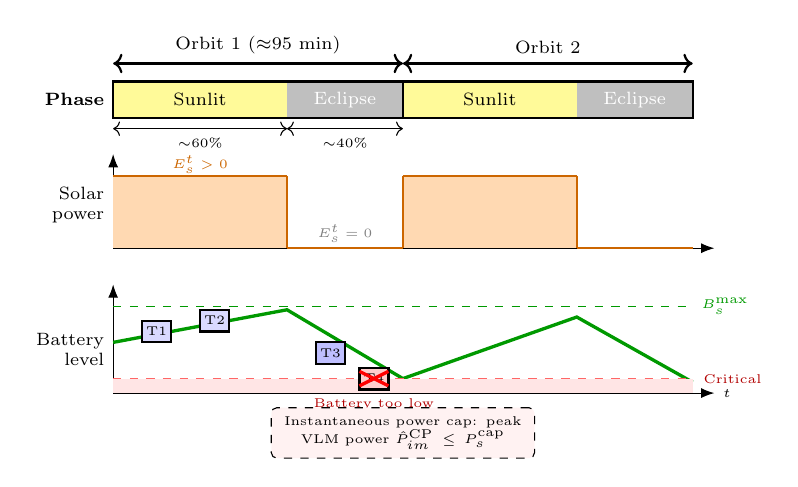
\begin{tikzpicture}[
  scale=0.92, every node/.style={scale=0.92},
]

% --- Time axis ---
\def\totalW{8.0}  % total width
\def\orbitW{4.0}  % one orbit width
\def\sunF{0.6}    % sunlit fraction
\def\eclF{0.4}    % eclipse fraction

% Row 1: Orbital phase bar (top)
\def\rowA{4.2}

% Orbit 1
\fill[yellow!40] (0, \rowA) rectangle (\orbitW*\sunF, \rowA+0.5);
\fill[gray!50] (\orbitW*\sunF, \rowA) rectangle (\orbitW, \rowA+0.5);
% Orbit 2
\fill[yellow!40] (\orbitW, \rowA) rectangle (\orbitW+\orbitW*\sunF, \rowA+0.5);
\fill[gray!50] (\orbitW+\orbitW*\sunF, \rowA) rectangle (2*\orbitW, \rowA+0.5);

\draw[thick] (0, \rowA) rectangle (\totalW, \rowA+0.5);
\draw[thick] (\orbitW, \rowA) -- (\orbitW, \rowA+0.5);

% Labels on bar
\node[font=\scriptsize] at (\orbitW*\sunF/2, \rowA+0.25) {Sunlit};
\node[font=\scriptsize, white] at (\orbitW*\sunF + \orbitW*\eclF/2, \rowA+0.25) {Eclipse};
\node[font=\scriptsize] at (\orbitW+\orbitW*\sunF/2, \rowA+0.25) {Sunlit};
\node[font=\scriptsize, white] at (\orbitW+\orbitW*\sunF + \orbitW*\eclF/2, \rowA+0.25) {Eclipse};

% Sun/moon icons
\node[font=\small] at (-0.4, \rowA+0.25) {};
\node[font=\scriptsize, left] at (0, \rowA+0.25) {\textbf{Phase}};

% Orbit period labels
\draw[<->, thick] (0, \rowA+0.75) -- (\orbitW, \rowA+0.75) node[midway, above, font=\scriptsize] {Orbit 1 ($\approx$95 min)};
\draw[<->, thick] (\orbitW, \rowA+0.75) -- (2*\orbitW, \rowA+0.75) node[midway, above, font=\scriptsize] {Orbit 2};

% 60/40 annotation
\draw[<->, thin] (0, \rowA-0.15) -- (\orbitW*\sunF, \rowA-0.15) node[midway, below, font=\tiny] {$\sim$60\%};
\draw[<->, thin] (\orbitW*\sunF, \rowA-0.15) -- (\orbitW, \rowA-0.15) node[midway, below, font=\tiny] {$\sim$40\%};

% --- Row 2: Solar power arrival ---
\def\rowB{2.4}
\node[font=\scriptsize, left, align=right] at (0, \rowB+0.6) {Solar\\power};

\draw[-Latex, thin] (0, \rowB) -- (0, \rowB+1.3);
\draw[-Latex, thin] (0, \rowB) -- (\totalW+0.3, \rowB);

% Sunlit: high solar, Eclipse: zero
% Orbit 1 sunlit
\fill[orange!30] (0, \rowB) rectangle (\orbitW*\sunF, \rowB+1.0);
\draw[thick, orange!80!black] (0, \rowB+1.0) -- (\orbitW*\sunF, \rowB+1.0);
\draw[thick, orange!80!black] (\orbitW*\sunF, \rowB+1.0) -- (\orbitW*\sunF, \rowB);
% Eclipse: zero
\draw[thick, orange!80!black] (\orbitW*\sunF, \rowB) -- (\orbitW, \rowB);
% Orbit 2 sunlit
\fill[orange!30] (\orbitW, \rowB) rectangle (\orbitW+\orbitW*\sunF, \rowB+1.0);
\draw[thick, orange!80!black] (\orbitW, \rowB) -- (\orbitW, \rowB+1.0);
\draw[thick, orange!80!black] (\orbitW, \rowB+1.0) -- (\orbitW+\orbitW*\sunF, \rowB+1.0);
\draw[thick, orange!80!black] (\orbitW+\orbitW*\sunF, \rowB+1.0) -- (\orbitW+\orbitW*\sunF, \rowB);
% Eclipse 2: zero
\draw[thick, orange!80!black] (\orbitW+\orbitW*\sunF, \rowB) -- (2*\orbitW, \rowB);

\node[font=\tiny, orange!80!black] at (\orbitW*\sunF/2, \rowB+1.15) {$E_s^t > 0$};
\node[font=\tiny, gray] at (\orbitW*\sunF + \orbitW*\eclF/2, \rowB+0.2) {$E_s^t = 0$};

% --- Row 3: Battery level ---
\def\rowC{0.4}
\node[font=\scriptsize, left, align=right] at (0, \rowC+0.6) {Battery\\level};

\draw[-Latex, thin] (0, \rowC) -- (0, \rowC+1.5);
\draw[-Latex, thin] (0, \rowC) -- (\totalW+0.3, \rowC) node[right, font=\tiny] {$t$};

% B_max line
\draw[dashed, thin, green!60!black] (0, \rowC+1.2) -- (\totalW, \rowC+1.2) node[right, font=\tiny] {$B_s^{\max}$};

% Battery curve: starts mid, charges during sunlit, discharges during eclipse
% Orbit 1: sunlit - charge from 0.6 to 1.0, eclipse - discharge from 1.0 to 0.35
% Orbit 2: sunlit - charge from 0.35 to 0.9, eclipse - discharge from 0.9 to 0.25
\draw[very thick, green!60!black]
  (0, \rowC+0.7) -- (\orbitW*\sunF, \rowC+1.15) -- (\orbitW, \rowC+0.2)
  -- (\orbitW+\orbitW*\sunF, \rowC+1.05) -- (2*\orbitW, \rowC+0.15);

% Danger zone
\fill[red!10] (0, \rowC) rectangle (\totalW, \rowC+0.2);
\draw[dashed, thin, red!60] (0, \rowC+0.2) -- (\totalW, \rowC+0.2);
\node[font=\tiny, red!70!black] at (\totalW+0.55, \rowC+0.2) {Critical};

% Inference task blocks on battery curve
\node[draw, fill=blue!15, thick, minimum width=4mm, minimum height=3mm, font=\tiny, inner sep=1pt] at (0.6, \rowC+0.85) {T1};
\node[draw, fill=blue!15, thick, minimum width=4mm, minimum height=3mm, font=\tiny, inner sep=1pt] at (1.4, \rowC+1.0) {T2};
\node[draw, fill=blue!25, thick, minimum width=4mm, minimum height=3mm, font=\tiny, inner sep=1pt] at (3.0, \rowC+0.55) {T3};
\node[draw, fill=red!20, thick, minimum width=4mm, minimum height=3mm, font=\tiny, inner sep=1pt] at (3.6, \rowC+0.2) {T4};

% Cross out T4 (cannot run - battery too low, at critical line)
\draw[red, very thick] (3.4, \rowC+0.1) -- (3.8, \rowC+0.3);
\draw[red, very thick] (3.4, \rowC+0.3) -- (3.8, \rowC+0.1);

% Annotation for T4
\node[font=\tiny, red!70!black, align=center] at (3.6, \rowC-0.15) {Battery too low};

% Power cap annotation (centered below battery plot)
\node[draw, dashed, rounded corners=2pt, fill=red!5, font=\tiny, align=center, text width=34mm] at (\totalW/2, \rowC-0.55) {Instantaneous power cap: peak VLM power $\hat{P}_{im}^{\text{CP}} \leq P_s^{\text{cap}}$};

\end{tikzpicture}
\caption{Energy challenges in solar-powered LEO satellite inference.  A satellite at 550\,km altitude experiences $\sim$60\% sunlit and $\sim$40\% eclipse per 95-minute orbit.  Solar power drops to zero during eclipse, forcing the battery to sustain all computation.  Tasks T1--T3 execute normally, but T4 is infeasible due to depleted battery.  Each slot must respect an instantaneous power cap $P_s^{\text{cap}}$.}
\label{fig:energy_motivation}
\end{figure}
%

% === Para 4: Gap — specific delta, not a laundry list ===
While~\cite{Zhang2025LEO} addresses collaborative VLM inference over LEO and~\cite{Luo2025SolarEdge} addresses solar-powered edge scheduling, neither handles the joint coupling of eclipse-induced energy intermittency and hardware peak-power caps that is central to on-orbit VLM deployment.  Terrestrial collaborative inference methods~\cite{Duan2024EdgeShard, Li2025TpiLLM} and on-device LLM optimizations~\cite{Xu2025EdgeLLM, He2024LLMOffload} assume unlimited energy and static networks, making them inapplicable to the LEO setting.

% === Para 5: Our approach (high-level, clear delta) ===
To the best of our knowledge, this is the first work to jointly address these coupled constraints.  We propose a two-timescale online framework: an offline stage determines VLM deployment across the constellation, and an online Lyapunov-based scheduler makes per-slot offloading and model-selection decisions using only current state, maximizing the minimum long-term inference quality across sensing sources (max-min fairness).  Two technical components enable this framework: a robust Lyapunov analysis based on input-to-state stability (ISS)~\cite{Huang2025RobustLyapunov} that preserves queue stability through zero-harvest eclipse intervals, and calibrated peak-power bounds obtained from offline hardware profiling that render per-slot power feasibility checkable in closed form.

% === Para 6: Contributions — novelty-first, result-oriented C4 ===
The main contributions are:
%
\begin{itemize}
    %
    \item[\bf C1.] \emph{First formulation} of energy-aware collaborative VLM inference over solar-powered LEO satellite networks, jointly capturing two-stage pipeline splitting across satellites, instantaneous peak-power caps, orbital eclipse dynamics, dynamic ISL topology, and max-min quality fairness.
    %
    \item[\bf C2.] \emph{A two-timescale robust Lyapunov framework} comprising an offline ILP for VLM deployment (including pipeline stage pairing) and a lightweight per-slot online scheduler, with calibrated power bounds that make peak-power feasibility checkable per slot.
    %
    \item[\bf C3.] \emph{Rigorous theoretical guarantees}: an $O(1/V)$ optimality gap, mean-rate constraint satisfaction under a Slater condition, and robust stability during eclipse via an ISS-based analysis that extends single-queue routing results to coupled energy--power queues.
    %
    \item[\bf C4.] \emph{Empirical validation} on EuroSAT~\cite{Helber2019EuroSAT} and RESISC45~\cite{Cheng2017RESISC45} with ViT-B/16 through ViT-G/14 at multiple quantization levels, showing that the proposed framework achieves zero peak-power violations while maintaining min-quality within a small gap of the offline MILP benchmark, compared to baselines that ignore one or more of the four constraints.
    %
\end{itemize}
%

The remainder of this paper is organized as follows.  Section~\ref{RWORKS} reviews related works.  Section~\ref{SYSMODEL} presents the system model and problem formulation.  Section~\ref{SOLUTION} describes the robust Lyapunov online optimization framework.  Section~\ref{ANALYSIS} provides theoretical analysis.  Section~\ref{EVAL} reports evaluation results, and Section~\ref{CONC} concludes the paper.
%


%%%%%%%%%%%%%%%%%%%%%%%%%%%%%%%%%%%%%%%%%%%%%%%%%%%%
\section{Related Works}\label{RWORKS}
%%%%%%%%%%%%%%%%%%%%%%%%%%%%%%%%%%%%%%%%%%%%%%%%%%%%
%
Our research overlaps with works that aim to (i) schedule AI inference tasks on energy-harvesting edge devices, (ii) split and distribute large models across multiple nodes for collaborative inference, and (iii) model the energy and power dynamics of neural network inference.
%

%
\begin{table*}[!t]
    \centering
\caption{A comparison of related works.}
\label{LR_Comp}
    \begin{threeparttable}
    \begin{tabular}{|c|c|c|c|c|c|c|c|c|} \hline
         \textbf{Ref.} & \textbf{\begin{tabular}{@{}c@{}}Energy \\ Harvesting\end{tabular}} & \textbf{\begin{tabular}{@{}c@{}}Model \\ Splitting\end{tabular}} & \textbf{\begin{tabular}{@{}c@{}}Activation \\ Compress.\end{tabular}} & \textbf{\begin{tabular}{@{}c@{}}Power Cap \\ Constraint\end{tabular}} & \textbf{\begin{tabular}{@{}c@{}}Online \\ Algorithm\end{tabular}} & \textbf{\begin{tabular}{@{}c@{}}Max-Min \\ Quality\end{tabular}} & \textbf{\begin{tabular}{@{}c@{}}LEO \\ Satellite\end{tabular}} & \textbf{\begin{tabular}{@{}c@{}}VLM\end{tabular}} \\ \hline
         %
         \cite{Mao2017MEC} & & & & & & & & \\ \hline
         %
         \cite{Mei2023Offloading, Khoshsirat2024DecentralizedEH} & \checkmark & & & & & & & \\ \hline
         %
         \cite{Luo2025SolarEdge} & \checkmark & & & & \checkmark & & & \\ \hline
         %
         \cite{Cheng2025TVT} & \checkmark & & & & \checkmark & & \checkmark & \\ \hline
         %
         \cite{Yao2025LEOEdge, Sun2026TVT} & & & & & & & \checkmark & \checkmark \\ \hline
         %
         \cite{Tang2024JSAC, Zhou2024MobilitySEC, Huang2025RobustLyapunov} & & & & & \checkmark & & \checkmark & \\ \hline
         %
         \cite{Zheng2024JSAC, Chen2025LEOUAV, Wu2026TVT} & & & & & & & \checkmark & \\ \hline
         %
         \cite{Xu2024DeViT, Lyu2025JSAC} & & \checkmark & & & & & & \checkmark \\ \hline
         %
         \cite{Dai2025CoopDNN} & & \checkmark & & & \checkmark & & & \\ \hline
         %
         \cite{Duan2024EdgeShard} & & \checkmark & & & & & & \\ \hline
         %
         \cite{Zhang2025LEO} & & \checkmark & \checkmark & & & & \checkmark & \checkmark \\ \hline
         %
         \cite{Xu2025EdgeLLM} & & & & & & & & \checkmark \\ \hline
         %
         \cite{He2024LLMOffload} & & & & & \checkmark & & & \checkmark \\ \hline
         %
         \cite{He2026LDDPG} & & & & & \checkmark & & & \\ \hline
         %
         {\bf Our Work} & \checkmark & \checkmark & \checkmark & \checkmark & \checkmark & \checkmark & \checkmark & \checkmark \\ \hline
         %
    \end{tabular}
    \end{threeparttable}
\end{table*}
%

%
\subsection{EH-Aware Edge AI Scheduling}\label{RW_EHA}
%
Mobile edge computing with energy harvesting (EH) has been studied extensively~\cite{Mao2017MEC}.  Mei et al.~\cite{Mei2023Offloading} and Luo et al.~\cite{Luo2025SolarEdge} optimize task offloading and workload scheduling for solar-powered edge servers, while Khoshsirat et al.~\cite{Khoshsirat2024DecentralizedEH} extend EH-aware scheduling to decentralized LLM inference.  For terrestrial EH networks, the solar energy arrival is commonly modeled by HMMs~\cite{Ku2015Solar}; in LEO, however, solar energy is governed by deterministic orbital mechanics rather than atmospheric conditions, requiring a different modeling approach.
%

%
In the LEO satellite domain, a range of works address computation offloading and resource allocation: mobility-aware offloading~\cite{Zhou2024MobilitySEC}, game-theoretic UAV-LEO offloading~\cite{Chen2025LEOUAV}, energy-constrained satellite-terrestrial scheduling~\cite{Cheng2025TVT}, inter-satellite cooperative caching~\cite{Wu2026TVT}, LLM-assisted resource allocation~\cite{Sun2026TVT}, satellite-ground cooperation platforms~\cite{Yao2025LEOEdge}, two-timescale service deployment~\cite{Tang2024JSAC}, and semantic communication for offloading~\cite{Zheng2024JSAC}.  However, none of these works jointly address collaborative VLM inference with model splitting, energy harvesting, or instantaneous power cap constraints.
%

%
\subsection{Collaborative Inference and Model Splitting}\label{RW_SPLIT}
%
When a model exceeds the memory of a single device, a natural solution is to split it across multiple nodes.  The Vision Transformer (ViT)~\cite{Dosovitskiy2021ViT} is particularly amenable to layer-wise partitioning due to its uniform block structure.  On terrestrial edge devices, DeViT~\cite{Xu2024DeViT} decomposes large ViTs for collaborative inference, EdgeShard~\cite{Duan2024EdgeShard} partitions LLMs across heterogeneous devices, Dai et al.~\cite{Dai2025CoopDNN} jointly optimize device placement and model partitioning with an online algorithm, Tpi-LLM~\cite{Li2025TpiLLM} serves 70B-scale LLMs via tensor parallelism, and Lyu et al.~\cite{Lyu2025JSAC} analyze the model-size vs.\ communication overhead trade-off.  For on-device inference, EdgeLLM~\cite{Xu2025EdgeLLM} employs speculative decoding and He et al.~\cite{He2024LLMOffload} study LLM offloading in cloud-edge computing.
%

%
In the satellite domain, Zhang et al.~\cite{Zhang2025LEO} split a ViT across multiple LEO satellites with pipeline parallelism and adaptive activation compression, validating on EuroSAT~\cite{Helber2019EuroSAT} and RESISC45~\cite{Cheng2017RESISC45}.  However, their formulation only minimizes inference delay and has no energy harvesting model, battery dynamics, or instantaneous power cap constraint.  Complementary to model splitting, SLICER~\cite{SLICER2025} proposes training-free activation compression that reduces transmitted volume by up to 10$\times$.
%

%
\subsection{Energy and Power Modeling for AI Inference}\label{RW_ENERGY}
%
Accurate energy and power models are essential for energy-aware scheduling.
%
Kasioulis et al.~\cite{Kasioulis2024EnergyModeling} benchmarked energy modeling of inference workloads with AI accelerators at the edge, revealing significant variance in power consumption across model architectures.
%
Husom et al.~\cite{Husom2025SustainableLLM} evaluated quantized LLMs for energy efficiency, and Xu et al.~\cite{Xu2025CAMEL} proposed an energy-aware LLM inference framework for resource-constrained devices.
%

%
A key observation is that neural network inference exhibits {\em phase-wise} power dynamics: GPU power ramps up during model loading, reaches a plateau during steady-state computation, and decays upon completion.
%
In this work, we profile each VLM configuration on the target hardware to extract calibrated instantaneous power bounds, which enter the optimization as offline-computed parameters.
%

%
\subsection{Lyapunov Optimization for Online Resource Management}\label{RW_LYAP}
%
Lyapunov optimization~\cite{Neely2010Lyapunov} decomposes long-term constrained problems into per-slot subproblems via virtual queues and drift-plus-penalty minimization, and has been applied to wireless resource allocation~\cite{Georgiadis2006Resource}, edge-cloud migration~\cite{Urgaonkar2015Dynamic}, and Lyapunov-guided deep RL for MEC~\cite{He2026LDDPG}.  In the LEO domain, Huang et al.~\cite{Huang2025RobustLyapunov} introduced a relaxed stability condition based on input-to-state stability (ISS), proving that the system remains stable as long as the overall Lyapunov drift trend is downward, even under temporary violations caused by bursty traffic or intermittent connectivity.  This robust framework is relevant to our setting, where eclipse periods disrupt energy supply.
%

%
\subsection{Discussion}\label{RW_DISC}
%
Table~\ref{LR_Comp} summarizes the comparison.  No prior work jointly addresses collaborative VLM inference with model splitting, solar energy harvesting with eclipse dynamics, instantaneous peak-power caps, dynamic ISL topology, and max-min quality fairness within an online optimization framework.  Our work fills this gap by unifying all eight dimensions in Table~\ref{LR_Comp}.
%


%%%%%%%%%%%%%%%%%%%%%%%%%%%%%%%%%%%%%%%%%%%%%%%%%%%%
\section{System Model and Problem Formulation}\label{SYSMODEL}
%%%%%%%%%%%%%%%%%%%%%%%%%%%%%%%%%%%%%%%%%%%%%%%%%%%%
%
We consider a LEO satellite constellation performing on-orbit Earth observation tasks using VLMs.  Fig.~\ref{fig:system_overview} illustrates the two collaborative 
inference topologies under sunlit and eclipse phases, and 
Table~\ref{notationTable} summarizes the key notations used 
throughout this paper.

%
\begin{figure*}[!t]
\centering
\includegraphics[width=\textwidth]{leo_system.pdf}
\caption{System overview of the LEO satellite network for collaborative 
VLM inference under sunlit and eclipse phases. (A)~Standalone topology, 
sunlit: sensing satellite uploads $D_i$ via ISL to a computing satellite 
running the full VLM. (B)~Standalone, eclipse: battery sustains 
inference without solar input. (C)~Split pipeline, sunlit: $D_i$ is 
forwarded to a front-stage satellite, which passes intermediate hidden 
states via ISL to a rear-stage satellite. (D)~Split pipeline, eclipse: 
both computing satellites rely on battery power; ISL connectivity must 
be maintained at the activation handoff slot $t + N_{im}$.}
\label{fig:system_overview}
\end{figure*}
%


%
\begin{table}[!t]
\small
\centering
\caption{\label{notationTable}A summary of notations.}
\begin{tabular}{lp{6.2cm}}
\toprule
{\bf 1.} & {\bf Sets} \\
\midrule
$\mathcal{T}$ & The set of discrete time slots, $|\mathcal{T}|$ is the planning horizon. \\
$\mathcal{S}$ & The set of computing satellites. \\
$\mathcal{I}$ & The set of sensing sources (sensing satellites). \\
$\mathcal{M}$ & The set of pre-enumerated VLM configurations ($\mathcal{M} = \mathcal{M}_S \cup \mathcal{M}_F \cup \mathcal{M}_R$). \\
$\mathcal{M}_S, \mathcal{M}_F, \mathcal{M}_R$ & Standalone, front-stage, and rear-stage configuration subsets. \\
$\pi(m)$ & Bijection mapping front stage $m \in \mathcal{M}_F$ to its rear stage in $\mathcal{M}_R$. \\
\midrule
{\bf 2.} & {\bf Parameters (offline-computed constants)} \\
\midrule
$\tau$ & Duration of a time slot. \\
$\lambda_i$ & Task arrival rate of source $i$. \\
$a_i^t$ & Task arrival indicator: $a_i^t = 1$ if source $i$ has a pending task at slot $t$. \\
$D_i$ & Data size of a task from source $i$ (in bits). \\
$Q_{im}$ & Inference quality of source $i$ under configuration $m$. \\
$\delta_s^t$ & Sunlit indicator: $\delta_s^t = 1$ if satellite $s$ 
is sunlit at slot $t$, $0$ during eclipse. \\
$\mathbb{E}[E_{im}]$ & Expected inference energy of source $i$ under configuration $m$. \\
$\mathbb{E}[T_{im}]$ & Expected inference time of source $i$ under configuration $m$. \\
$N_{im}$ & Number of slots required: $N_{im} = \lceil \mathbb{E}[T_{im}] / \tau \rceil$. \\
$\hat{P}_{im}^{\text{CP}}$ & Calibrated power upper bound for source $i$ under configuration $m$. \\
$P_s^{\text{cap}}$ & Hardware instantaneous power cap of satellite $s$. \\
$B_s^{\max}$ & Battery capacity of satellite $s$. \\
$R_s^{\max}$ & Memory (RAM) capacity of satellite $s$. \\
$R_m$ & Memory (RAM) requirement of VLM configuration $m$. \\
$L_m$ & Number of front-stage layers in split config $m \in \mathcal{M}_F$. \\
$E_s^t$ & Solar energy arrival at satellite $s$ in slot $t$. \\
$\omega_s^t$ & Energy actually stored: $\omega_s^t = \min(E_s^t, B_s^{\max} - b_s^t)$. \\
$C_{is}^t$ & ISL capacity between source $i$ and satellite $s$ in slot $t$ ($= 0$ if no path). \\
$\ell_{ss'}^t$ & ISL connectivity indicator between computing satellites $s$ and $s'$ at slot $t$. \\
$d_{is}^t$ & Inter-satellite distance from source $i$ to satellite $s$ in slot $t$. \\
$P_{\text{tx}}$ & Transmit power. \\
$G_{\text{tx}}, G_{\text{rx}}$ & Transmit and receive antenna gains. \\
$f$ & Carrier frequency. \\
$k_B T_{\text{sys}}$ & System noise power spectral density. \\
$W$ & Bandwidth of the inter-satellite link. \\
\midrule
{\bf 3.} & {\bf Decision Variables} \\
\midrule
$\alpha_{is}^t$ & Whether source $i$'s task is uploaded to satellite $s$ in slot $t$ (binary). \\
$y_{sm}$ & Whether satellite $s$ is configured with VLM configuration $m$ (binary). \\
$x_{ism}^t$ & Whether source $i$'s task starts execution on $(s, m)$ in slot $t$ (binary). \\
\midrule
{\bf 4.} & {\bf Derived / State Variables} \\
\midrule
$z_{ism}^t$ & Execution indicator: source $i$ executing on $(s, m)$ in slot $t$ (from $x$ via~\eqref{C6a}). \\
$b_s^t$ & Battery level of satellite $s$ at the start of slot $t$. \\
$q_i^t$ & Inference quality delivered to source $i$ in slot $t$: $q_i^t = \sum_{s,m} x_{ism}^t Q_{im}$. \\
$\bar{q}_i$ & Long-term average quality of source $i$: $\bar{q}_i = \lim_{T\to\infty} \frac{1}{T}\sum_t \mathbb{E}[q_i^t]$. \\
\bottomrule
\end{tabular}
\end{table}


%  HTJ sensing satellites 跟 LEO 是同轨道还是异轨道？
% zjf 感知卫星与计算卫星的轨道关系没有固定，可以同轨道，也可以异轨道

\subsection{Network and VLM Configuration Model}\label{SM_NET}

The constellation comprises two types of satellites: a set $\mathcal{S}$ 
of computing satellites and a set $\mathcal{I}$ of sensing satellites. 
This partition reflects the heterogeneous nature of LEO constellations, 
where earlier-generation satellites with limited onboard compute serve 
as sensing nodes, while newer satellites with dedicated accelerators 
host VLM inference workloads. Each computing satellite $s \in \mathcal{S}$ 
is equipped with a solar panel, a rechargeable battery with capacity 
$B_s^{\max}$, and an onboard computing platform with RAM capacity 
$R_s^{\max}$. Each sensing satellite $i \in \mathcal{I}$ generates 
observation tasks at rate $\lambda_i$; let $a_i^t \in \{0,1\}$ indicate 
whether source $i$ has a pending task at slot $t$, with data size $D_i$. 
We consider a planning horizon of $|\mathcal{T}|$ discrete time slots, 
each of duration $\tau$. Each satellite hosts at most one VLM 
configuration $y_{sm} \in \{0,1\}$ for the entire horizon:
%
\begin{eqnarray}\label{C4a}
\sum_{m \in \mathcal{M}} y_{sm} \leq 1, \quad \forall s \in \mathcal{S},
\end{eqnarray}
%
\begin{eqnarray}\label{C9}
\sum_{m \in \mathcal{M}} y_{sm} \cdot R_m \leq R_s^{\max}, \quad 
\forall s \in \mathcal{S}.
\end{eqnarray}

The VLM configuration set $\mathcal{M} = \mathcal{M}_S \cup \mathcal{M}_F 
\cup \mathcal{M}_R$ contains standalone configurations ($\mathcal{M}_S$, 
full model on one satellite), front-stage configurations ($\mathcal{M}_F$, 
first $L_m$ transformer blocks), and rear-stage configurations 
($\mathcal{M}_R$, remaining blocks). A bijection $\pi\!: \mathcal{M}_F 
\!\to\! \mathcal{M}_R$ pairs each front stage with its rear counterpart. 
Each configuration $m$ specifies the VLM architecture, quantization 
level, layer range, and activation compression bit-width for ISL 
transmission. Because ViT blocks are identical, the intermediate 
activation size is constant regardless of the split point~\cite{Zhang2025LEO}, 
and activation transfer at laser-ISL rates is negligible compared with 
inference latency. A task executes on satellite $s$ only if $y_{sm}=1$, 
and for a split pipeline both stages must be deployed:
%
\begin{eqnarray}\label{C4b}
x_{ism}^t \leq y_{sm}, \quad \forall i,\, s,\, m,\, t,
\end{eqnarray}
%
\begin{eqnarray}\label{C_deploy_pipe}
y_{sm} \leq \sum_{s' \in \mathcal{S}} y_{s',\pi(m)}, \quad 
\forall s \in \mathcal{S},\, \forall m \in \mathcal{M}_F.
\end{eqnarray}

For each pair $(i, m)$, the expected energy $\mathbb{E}[E_{im}]$, 
execution time $\mathbb{E}[T_{im}]$, calibrated power bound 
$\hat{P}_{im}^{\text{CP}}$, and required slots $N_{im} = \lceil 
\mathbb{E}[T_{im}] / \tau \rceil$ are computed offline. The inference 
quality $Q_{im}$ denotes the task-specific accuracy of configuration 
$m$ on tasks from source $i$ (e.g., determined by land-cover category); 
it equals the full-pipeline accuracy for $m \in \mathcal{M}_S \cup 
\mathcal{M}_R$ and is zero for $m \in \mathcal{M}_F$, since quality 
is attributed entirely to the rear stage $\pi(m)$.
%
\subsection{Communication and Task Offloading}\label{SM_COMM}
%
%ZJF 
% 拓扑结构目前是每颗卫星维持 4 条星间链路，2 条 intra-plane 链路（同轨道平面内）固定的， 2 条 inter-plane 链路（跨轨道平面）会随着time slot变化，这个设定来自于kwan的那篇safe rl的卫星论文，但我们不同的是跨轨道的拓扑结构的变化想来源于真实的卫星数据比如spacex的数据来设定，这个是随着轨道而变化的受轨道力学调控，所以要首先搞清楚这个变化的时间尺度和我们slot的，vlm推理时间尺度是否合理
% 计划采用真实 TLE/星历离线预计算的轨道力学外生动态 ISL 拓扑(同轨道固定、跨轨道随时隙变化),据此区分三个时间尺度——分钟级的阳照/地影能量周期、几十秒级的拓扑相干窗口、以及秒级的 VLM 推理调度时隙 τ,并通过在 Jetson Orin NX 上用 EuroSAT 实测各 VLM 配置的单次推理时长来确定 τ 及对应的 N_im,使三个尺度层层分离、互不冲突。


Following the standard +Grid ISL topology adopted in LEO constellations~\cite{Huang2025RobustLyapunov, Yi2025FSO}, each satellite maintains four inter-satellite links: two \emph{intra-plane} links connecting the adjacent satellites in the same orbit, and two \emph{inter-plane} links connecting satellites in neighboring orbital planes.  Intra-plane neighbors are fixed because satellites in the same orbit share identical ground tracks.  Inter-plane neighbors, however, change over time as satellites in different orbital planes move at different angular velocities; within each slot the topology is treated as static, but the inter-plane connectivity may differ across slots.  When no ISL path exists between source~$i$ and satellite~$s$ at slot~$t$, we set $C_{is}^t = 0$.

Modern LEO constellations increasingly employ free-space optical (laser) ISLs~\cite{Yi2025FSO}, which operate with a clear line-of-sight path and no multipath scattering.  We therefore adopt a free-space path loss (FSPL) model.  The received signal-to-noise ratio between the sensing satellite of source $i$ and computing satellite $s$ in slot $t$ is
%
\begin{eqnarray}\label{channel_gain}
\text{SNR}_{is}^t = \frac{P_{\text{tx}} \, G_{\text{tx}} \, G_{\text{rx}}}{k_B \, T_{\text{sys}} \, W} \cdot \left(\frac{c}{4\pi f \, d_{is}^t}\right)^2,
\end{eqnarray}
%
where $P_{\text{tx}}$ is the transmit power, $G_{\text{tx}}$ and $G_{\text{rx}}$ are the transmit and receive antenna gains, $k_B$ is the Boltzmann constant, $T_{\text{sys}}$ is the system noise temperature, $W$ is the bandwidth, $c$ is the speed of light, $f$ is the carrier frequency, and $d_{is}^t$ is the distance between the two satellites in slot $t$.  The inter-satellite distance $d_{is}^t$ varies over time due to orbital dynamics.  The link capacity is
%
\begin{eqnarray}\label{link_capacity}
C_{is}^t = W \log_2\!\left(1 + \text{SNR}_{is}^t\right).
\end{eqnarray}

Let $\ell_{ss'}^t \in \{0,1\}$ denote whether computing satellites $s$ and $s'$ are ISL-connected at slot~$t$.  This indicator is computable offline from orbital ephemeris data and is needed for activation handoff in pipeline execution (Section~\ref{SM_SCHED}).

Let $\alpha_{is}^t \in \{0,1\}$ denote whether the task from source $i$ is uploaded to satellite $s$ in slot $t$.  Each task is uploaded at most once, and the upload must fit within a single slot:
%
\begin{eqnarray}\label{C3a}
\sum_{s \in \mathcal{S}} \sum_{t \in \mathcal{T}} \alpha_{is}^t \leq 1, \quad \forall i \in \mathcal{I},
\end{eqnarray}
%
\begin{eqnarray}\label{C3b}
\alpha_{is}^t \cdot D_i \leq C_{is}^t \cdot \tau, \quad \forall i \in \mathcal{I},\, \forall s \in \mathcal{S},\, \forall t \in \mathcal{T}.
\end{eqnarray}
%

%
\subsection{Task Scheduling}\label{SM_SCHED}
%
Let $x_{ism}^t \in \{0,1\}$ denote whether the task from source $i$ 
starts execution on satellite $s$ with configuration $m$ at slot $t$. 
Each task is processed at most once; to avoid double-counting, we 
restrict the at-most-once constraint to standalone or front-stage 
starts, since the rear-stage execution is jointly determined by the 
pipeline coupling and precedence constraints \eqref{C_pipe_couple}--
\eqref{C_pipe_prec}. Specifically, $x_{is',\pi(m)}^t$ remains a 
decision variable because multiple satellites may host the rear-stage 
configuration, and the scheduler must select which one to use subject 
to ISL connectivity \eqref{C_pipe_isl}:
%
\begin{eqnarray}\label{C2}
\sum_{s \in \mathcal{S}} \sum_{m \in \mathcal{M}_S \cup \mathcal{M}_F} 
\sum_{t \in \mathcal{T}} x_{ism}^t \leq 1, \quad \forall i \in \mathcal{I}.
\end{eqnarray}
%
Execution of a standalone or front-stage configuration can start 
only after the task data has been uploaded to the same
satellite $s$, ensuring that the upload destination and the 
execution host coincide:
%
\begin{eqnarray}\label{C5}
x_{ism}^t \leq \sum_{k=1}^{t} \alpha_{is}^k, \quad \forall i,\, s,\, m \in \mathcal{M}_S \cup \mathcal{M}_F,\, t.
\end{eqnarray}
%
A rear-stage configuration receives intermediate activations via ISL rather than raw data, so its prerequisite is the precedence constraint~\eqref{C_pipe_prec} instead of~\eqref{C5}.

Once started, a task runs non-preemptively for $N_{im}$ consecutive slots.  The execution indicator $z_{ism}^t \in \{0,1\}$ is fully determined by the start variables:
%
\begin{eqnarray}\label{C6a}
z_{ism}^t = \sum_{t'=\max(1,\, t-N_{im}+1)}^{t} x_{ism}^{t'}, \quad \forall i,s,m,t.
\end{eqnarray}
%
At most one task per (satellite, configuration) at any time:
%
\begin{eqnarray}\label{C6b}
\sum_{i \in \mathcal{I}} z_{ism}^t \leq 1, \quad \forall s \in \mathcal{S},\, \forall m \in \mathcal{M},\, \forall t \in \mathcal{T}.
\end{eqnarray}
%
All tasks must complete within the horizon:
%
\begin{eqnarray}\label{C11}
x_{ism}^t \cdot (t + N_{im} - 1) \leq |\mathcal{T}|, \quad \forall i,s,m,t.
\end{eqnarray}
%

For split configurations, starting a front stage commits the system 
to executing the corresponding rear stage. Specifically, if a front 
stage is scheduled, the corresponding rear stage must also be 
scheduled:
%
\begin{eqnarray}\label{C_pipe_couple}
\sum_{s} \sum_{t} x_{is,\pi(m)}^t = \sum_{s} \sum_{t} x_{ism}^t, 
\;\; \forall i \in \mathcal{I},\, m \in \mathcal{M}_F.
\end{eqnarray}
%
The rear stage starts immediately after the front stage completes 
(activation transfer is negligible at laser-ISL rates):
%
\begin{eqnarray}\label{C_pipe_prec}
x_{is',\pi(m)}^{t'} \leq \sum_{s \in \mathcal{S}} x_{ism}^{t'-N_{im}}, 
\;\; \forall i,\, s',\, m \in \mathcal{M}_F,\, t'.
\end{eqnarray}
%
Since activations are transferred via ISL at handoff, the front- and 
rear-stage satellites must be ISL-connected at that moment:
%
\begin{eqnarray}\label{C_pipe_isl}
x_{ism}^t + x_{is',\pi(m)}^{t+N_{im}} \leq 1 + \ell_{ss'}^{t+N_{im}}, 
\nonumber \\
\forall i,\, s,\, s',\, m \in \mathcal{M}_F,\, t.
\end{eqnarray}
%

%
\subsection{Energy and Resource Constraints}\label{SM_ENERGY}
%
Each satellite $s$ harvests solar energy. Unlike terrestrial settings 
where weather introduces multi-state stochasticity~\cite{Ku2015Solar}, 
LEO solar energy is governed by orbital mechanics: a satellite at 
altitude $h$ follows a periodic orbit of period $T_{\text{orb}}$, 
spending a fraction $f_{\text{sun}}$ in sunlight and $1-f_{\text{sun}}$ 
in eclipse. Let $\delta_s^t \in \{0,1\}$ 
denote the sunlit indicator of satellite $s$ at slot $t$, where 
$\delta_s^t = 1$ if the satellite is in sunlight and $\delta_s^t = 0$ 
during eclipse; this indicator is deterministic and computable offline 
from two-line element (TLE) data. We model the solar energy arrival as
%
\begin{eqnarray}\label{solar_model}
E_s^t = P_{\text{solar}} \cdot (\eta_s + \epsilon_s^t) \cdot \tau 
\cdot \delta_s^t,
\end{eqnarray}
%
where $P_{\text{solar}}$ is the solar irradiance at the panel, $\eta_s$ 
is the panel efficiency, and $\mathbbm{1}[\cdot]$ is the sunlit indicator 
determined by the orbital ephemeris.  The sunlit/eclipse transition is 
periodic and predictable from two-line element (TLE) data; we add a small 
random perturbation $\epsilon_s^t \sim \mathcal{N}(0, \sigma_\eta^2)$ to 
$\eta_s$ to account for attitude variations and panel degradation.
%
\begin{eqnarray}\label{C7a}
0 \leq \omega_s^t \leq E_s^t, \quad \forall s \in \mathcal{S},\, \forall t \in \mathcal{T}, \\
\label{C7b}
b_s^t + \omega_s^t \leq B_s^{\max}, \quad \forall s \in \mathcal{S},\, \forall t \in \mathcal{T}.
\end{eqnarray}
%
The battery level evolves as
%
\begin{eqnarray}\label{C7c}
b_s^{t+1} = b_s^t + \omega_s^t - \sum_{i,m} z_{ism}^t \cdot \frac{\mathbb{E}[E_{im}]}{N_{im}}, \quad \forall s,t.
\end{eqnarray}
%
The battery level is non-negative, and energy consumption cannot exceed available energy in any slot:
%
\begin{eqnarray}\label{C7d}
\sum_{i,m} z_{ism}^t \cdot \frac{\mathbb{E}[E_{im}]}{N_{im}} \leq b_s^t + \omega_s^t, \quad \forall s,t, \\
\label{C7e}
b_s^t \geq 0, \quad \forall s \in \mathcal{S},\, \forall t \in \mathcal{T}.
\end{eqnarray}
%
The instantaneous power cap requires that the total power draw never exceeds the hardware limit:
%
\begin{eqnarray}\label{C8}
\sum_{i,m} z_{ism}^t \cdot \hat{P}_{im}^{\text{CP}} \leq P_s^{\text{cap}}, \quad \forall s,t.
\end{eqnarray}

The calibrated power bound $\hat{P}_{im}^{\text{CP}}$ is obtained 
by offline hardware profiling: for each configuration $m$, we 
record the instantaneous power trace and extract a high quantile 
of the peak power distribution, since VLM inference exhibits 
phase-wise power dynamics that cause instantaneous power to 
significantly exceed the average.

%
\subsection{Problem Formulation}\label{SM_OBJ}
%
Our objective is to maximize the minimum inference quality across all sensing sources.  We jointly optimize (i) task offloading decisions, (ii) VLM configuration deployment, (iii) task scheduling, (iv) energy management, and (v) quality assurance.

Let $q_i^t = \sum_{s,m} x_{ism}^t \cdot Q_{im}$ denote the inference quality delivered to source $i$ in slot $t$.  Since $Q_{im} = 0$ for all $m \in \mathcal{M}_F$, quality is credited only when a standalone configuration completes or a rear stage starts, which is exactly when the full VLM inference result becomes available.  Define the long-term average quality per source as $\bar{q}_i = \lim_{T \to \infty} \frac{1}{T} \sum_{t=1}^{T} \mathbb{E}[q_i^t]$.  The stochastic optimization problem is:
%
\begin{align}
\max_{\boldsymbol{\pi}} \quad & \min_{i \in \mathcal{I}} \; \bar{q}_i \tag{$\mathbf{P}$} \label{P_stoch} \\[3pt]
\text{s.t.} \quad & \eqref{C4a}\mbox{-}\eqref{C_pipe_isl}, \nonumber \\
& \lim_{T \to \infty} \frac{1}{T} \sum_{t=1}^{T} \mathbb{E}\!\left[\sum_{i,m} z_{ism}^t \frac{\mathbb{E}[E_{im}]}{N_{im}} - \omega_s^t\right] \leq 0, \; \forall s, \label{C_longE}\\
& \sum_{i,m} z_{ism}^t \cdot \hat{P}_{im}^{\text{CP}} \leq P_s^{\text{cap}}, \; \forall s, t, \label{C_pcap}
\end{align}
%
where $\boldsymbol{\pi} = [\alpha_{is}^t, y_{sm}, x_{ism}^t]$ denotes the collection of all decision variables ($z_{ism}^t$ is determined by $x$ via~\eqref{C6a}).  The objective maximizes the minimum long-term average quality across all sensing sources.  Constraint~\eqref{C_longE} enforces a long-term average energy budget at each satellite, and~\eqref{C_pcap} enforces the per-slot instantaneous power cap using calibrated power bounds.  The energy and power sums in~\eqref{C_longE}--\eqref{C_pcap} naturally account for both standalone and pipeline executions: a satellite hosting a front stage incurs the front-stage energy and power during its execution window, while the rear-stage satellite incurs the corresponding rear-stage costs.

Problem~\eqref{P_stoch} is a long-term stochastic optimization that couples decisions across time through battery dynamics, non-preemptive scheduling, and pipeline precedence constraints.  It involves both binary decision variables ($\alpha_{is}^t, y_{sm}, x_{ism}^t$) and continuous state variables ($b_s^t$); when all future information is known, it reduces to a finite-horizon mixed-integer linear program (MILP).  Solving the stochastic version directly requires full distributional knowledge and suffers from the curse of dimensionality, as the total number of binary variables scales as $O(|\mathcal{I}| \cdot |\mathcal{S}|^2 \cdot |\mathcal{M}| \cdot |\mathcal{T}|)$ (the $|\mathcal{S}|^2$ factor arises from pipeline satellite pairs).  In the next section, we develop an online algorithm that avoids these difficulties.


%%%%%%%%%%%%%%%%%%%%%%%%%%%%%%%%%%%%%%%%%%%%%%%%%%%%
\section{Robust Lyapunov Online Optimization}\label{SOLUTION}
%%%%%%%%%%%%%%%%%%%%%%%%%%%%%%%%%%%%%%%%%%%%%%%%%%%%
%
In this section, we design an online algorithm based on Lyapunov drift-plus-penalty~\cite{Neely2010Lyapunov} that decomposes the long-term problem~\eqref{P_stoch} into per-slot subproblems without requiring future information.  We further introduce a robust extension inspired by~\cite{Huang2025RobustLyapunov} to handle the intermittent energy supply caused by eclipse periods.

As a performance reference, we define an offline MILP benchmark that assumes full future knowledge.  By introducing an auxiliary variable $U$ to linearize the max-min objective, the offline formulation is:
%
\begin{align}
\max_{\boldsymbol{\pi}, U} \quad & U \tag{$\mathbf{P}_{\text{off}}$} \label{MILP_full} \\[3pt]
\text{s.t.} \quad & \eqref{C4a}\mbox{-}\eqref{C_pipe_isl}, \nonumber \\
& U \leq \sum_{s,m,t} x_{ism}^t \cdot Q_{im}, \quad \forall i \in \mathcal{I}. \label{C1}
\end{align}
%
This is a pure MILP because all energy and power parameters are precomputed offline.  It serves as an upper bound on the achievable performance of any online algorithm.  We use it in Section~\ref{ANALYSIS} to characterize the optimality gap.

%
\subsection{Two-Timescale Decomposition}\label{SOL_DECOMP}
%
We observe that problem~\eqref{P_stoch} has a natural two-timescale structure.  The model deployment decision $y_{sm}$ determines which VLM configuration is loaded on each satellite.  Loading a model into GPU memory is costly, so $y_{sm}$ remains fixed over the planning horizon.  In contrast, the task offloading $\alpha_{is}^t$ and scheduling $x_{ism}^t$ decisions must be made in each time slot under stochastic arrivals.

We exploit this structure by decomposing the problem into two levels.

\subsubsection{Upper Level --- Offline Model Deployment}
Given the statistical characteristics of task arrivals and solar energy, we solve a small-scale integer program to determine the model deployment:
%
\begin{align}
\max_{\{y_{sm}\}} \quad & \sum_{s \in \mathcal{S}} \sum_{m \in \mathcal{M}} y_{sm} \cdot \bar{Q}_m \label{upper_ILP} \\[3pt]
\text{s.t.} \quad & \sum_{m \in \mathcal{M}} y_{sm} \leq 1, \quad \forall s \in \mathcal{S}, \nonumber \\
& \sum_{m \in \mathcal{M}} y_{sm} \cdot R_m \leq R_s^{\max}, \quad \forall s \in \mathcal{S}, \nonumber \\
& y_{sm} \leq \textstyle\sum_{s'} y_{s',\pi(m)}, \quad \forall s \in \mathcal{S},\, m \in \mathcal{M}_F, \nonumber
\end{align}
%
where $\bar{Q}_m = \frac{1}{|\mathcal{I}|}\sum_{i} Q_{im}$ is the average quality of configuration $m$ across sources (note that $\bar{Q}_m = 0$ for $m \in \mathcal{M}_F$, so the objective naturally rewards deploying rear stages and standalone configurations, while the pipeline coupling constraint ensures that front stages are co-deployed).  This problem has $|\mathcal{S}| \cdot |\mathcal{M}|$ binary variables and can be solved efficiently.  Once $y_{sm}$ is fixed, the set of feasible configurations at each satellite is determined for the entire horizon.

\subsubsection{Lower Level --- Online Per-Slot Scheduling}
Given the model deployment $\{y_{sm}\}$, the remaining decisions $\alpha_{is}^t$ and $x_{ism}^t$ are made online in each slot $t$ using the Lyapunov drift-plus-penalty framework described below.

%
\subsection{Virtual Queue Design}\label{SOL_VQ}
%
The key idea of Lyapunov optimization is to convert long-term constraints into virtual queues whose stability implies constraint satisfaction~\cite{Neely2010Lyapunov}.  We introduce three types of virtual queues.

\subsubsection{Energy Virtual Queue}
For each satellite $s \in \mathcal{S}$, we define a virtual queue $Q_s^E(t)$ that tracks the cumulative energy deficit:
%
\begin{eqnarray}\label{vq_energy}
Q_s^E(t\!+\!1) = \max\!\left\{Q_s^E(t) + \sum_{i,m} z_{ism}^t \frac{\mathbb{E}[E_{im}]}{N_{im}} - \omega_s^t,\; 0\right\}\!,
\end{eqnarray}
%
where $Q_s^E(0) = 0$.  When the energy consumed exceeds the energy harvested, the queue backlog grows; when solar energy is abundant, it decreases.  Stabilizing $Q_s^E(t)$ in the mean-rate sense ensures the long-term energy budget constraint~\eqref{C_longE} is satisfied.

\subsubsection{Power Cap Virtual Queue}
For each satellite $s \in \mathcal{S}$, we define a virtual queue $Q_s^P(t)$ that tracks instantaneous power cap violations:
%
\begin{eqnarray}\label{vq_power}
Q_s^P(t\!+\!1) = \max\!\left\{Q_s^P(t) + \sum_{i,m} z_{ism}^t \hat{P}_{im}^{\text{CP}} - P_s^{\text{cap}},\; 0\right\}\!,
\end{eqnarray}
%
where $Q_s^P(0) = 0$.  The calibrated power bound $\hat{P}_{im}^{\text{CP}}$ (obtained via offline profiling, see Section~\ref{SM_ENERGY}) enters directly into this queue.

\subsubsection{Quality Deficit Virtual Queue}
For each sensing source $i \in \mathcal{I}$, we define a virtual queue $Q_i^U(t)$ that tracks the gap between the target quality level $U^{\text{tgt}}$ and the achieved quality:
%
\begin{eqnarray}\label{vq_quality}
Q_i^U(t\!+\!1) = \max\!\left\{Q_i^U(t) + a_i^t \cdot U^{\text{tgt}} - q_i^t,\; 0\right\}\!,
\end{eqnarray}
%
where $a_i^t \in \{0,1\}$ is the task arrival indicator and $U^{\text{tgt}}$ is an adjustable quality target.  The arrival indicator ensures that the queue grows only when source $i$ has a pending task; once the task is processed, $q_i^t = Q_{im} > 0$ provides a credit.  Stabilizing this queue ensures that each source's average quality meets the target.

Fig.~\ref{fig:lyapunov_framework} illustrates the online scheduling loop.

%
\begin{figure}[!t]
\centering
\definecolor{acblue}{RGB}{218,232,252}    % muted academic blue
\definecolor{acbluedark}{RGB}{70,130,180}  % steel blue for borders
\definecolor{acgrey}{RGB}{240,240,245}     % light grey
\definecolor{acgreydark}{RGB}{120,120,140} % slate grey for borders
\definecolor{acgreen}{RGB}{225,245,230}    % very light green
\definecolor{feedblue}{RGB}{50,100,170}    % feedback arrow
\resizebox{0.88\columnwidth}{!}{%
\begin{tikzpicture}[
  block/.style={draw=acbluedark, rounded corners=2pt, thick,
    minimum width=26mm, minimum height=9.5mm, align=center,
    font=\scriptsize},
  sblock/.style={draw=acgreydark, rounded corners=2pt, semithick,
    minimum width=22mm, minimum height=8.5mm, align=center,
    font=\scriptsize},
  arr/.style={-Latex, semithick, color=black!75},
  fbarr/.style={-Latex, semithick, color=feedblue, densely dashed},
]

% --- Row 0: title ---
\node[font=\small\bfseries] (title) at (1.9, 0.75) {Each slot $t$};

% --- Row 1: Observe State + Virtual Queues (same y, symmetric about centre) ---
\node[block, fill=acblue] (obs) at (0, 0)
  {\textbf{Observe State}\\[1pt] $\mathcal{I}_t,\; C_{is}^t,\; E_s^t$};
\node[block, fill=acblue] (vq) at (3.8, 0)
  {\textbf{Virtual Queues}\\[1pt] $Q_s^E(t),\; Q_s^P(t),\; Q_i^U(t)$};

% --- Row 2: Energy Params (left) + Min DPP (centre) ---
\node[sblock, fill=acgrey] (cape) at (-2.0, -1.55)
  {\textbf{Energy Params}\\[1pt] $\hat{P}_{im}^{\mathrm{CP}},\;\mathbb{E}[E_{im}]$};
\node[block, fill=acgreen] (dpp) at (1.9, -1.55)
  {\textbf{Min DPP}\\[1pt] $\Delta_V\!=\!\Delta(\mathbf{Q}(t)) - V\!\cdot\!\mathbb{E}[\sum_i q_i^t]$};

% --- Row 3: Per-Slot Solver ---
\node[block, fill=acblue!60] (solve) at (1.9, -3.05)
  {\textbf{Per-Slot Solver}\\[1pt] $\alpha_{is}^t,\; x_{ism}^t$};

% --- Row 4: Execute & Update ---
\node[block, fill=acgrey] (exec) at (1.9, -4.55)
  {\textbf{Execute \& Update}\\[1pt] Batteries, Queues};

% ===== Arrows =====
% Top row
\draw[arr] (obs) -- (vq);
% Into DPP: direct diagonal lines, no detour
\draw[arr] (obs.south) -- (dpp.north west);
\draw[arr] (vq.south) -- (dpp.north east);
\draw[arr] (cape.east) -- (dpp.west) node[midway, above, font=\tiny, inner sep=1pt] {$V$};
% Central vertical flow
\draw[arr] (dpp) -- (solve);
\draw[arr] (solve) -- (exec);

% Feedback loop (right side, dashed, single vertical line)
\coordinate (fbr) at ([xshift=8mm]vq.east);
\draw[fbarr] (exec.east) -| (fbr) -- (vq.east);
\node[font=\scriptsize, color=feedblue, left, inner sep=1pt] at (fbr|-solve) {$\mathbf{Q}(t\!+\!1)$};

\end{tikzpicture}%
}
\caption{Schematic of the online scheduling loop (lower level).  In each slot~$t$, the scheduler monitors the system state and virtual queue backlogs to formulate the drift-plus-penalty (DPP) objective.  Using pre-computed energy parameters, the framework solves a lightweight per-slot optimization, executes the control decisions, and updates queue states for the subsequent slot.}
\label{fig:lyapunov_framework}
\end{figure}

%
\subsection{Lyapunov Drift-Plus-Penalty}\label{SOL_DPP}
%
Define the aggregate virtual queue vector $\mathbf{Q}(t) = \{Q_s^E(t), Q_s^P(t), Q_i^U(t)\}_{s \in \mathcal{S}, i \in \mathcal{I}}$ and the quadratic Lyapunov function:
%
\begin{eqnarray}\label{lyap_func}
L(\mathbf{Q}(t)) = \frac{1}{2}\sum_{s \in \mathcal{S}} \left[(Q_s^E(t))^2 + (Q_s^P(t))^2\right] + \frac{1}{2}\sum_{i \in \mathcal{I}} (Q_i^U(t))^2.
\end{eqnarray}
%
The one-slot conditional Lyapunov drift is:
%
\begin{eqnarray}\label{lyap_drift}
\Delta(\mathbf{Q}(t)) = \mathbb{E}\left[L(\mathbf{Q}(t+1)) - L(\mathbf{Q}(t)) \mid \mathbf{Q}(t)\right].
\end{eqnarray}
%
By the standard Lyapunov technique, $\Delta(\mathbf{Q}(t))$ can be upper-bounded as follows.  Using the fact that $(\max\{a+b, 0\})^2 \leq a^2 + b^2 + 2ab$ for all $a, b$, we obtain
%
\begin{eqnarray}\label{drift_bound}
\Delta(\mathbf{Q}(t)) &\leq& B + \sum_{s} Q_s^E(t) \, \mathbb{E}\!\left[e_s^t - \omega_s^t \mid \mathbf{Q}(t)\right] \nonumber \\
&& + \sum_{s} Q_s^P(t) \, \mathbb{E}\!\left[p_s^t - P_s^{\text{cap}} \mid \mathbf{Q}(t)\right] \nonumber \\
&& + \sum_{i} Q_i^U(t) \, \mathbb{E}\!\left[a_i^t U^{\text{tgt}} - q_i^t \mid \mathbf{Q}(t)\right],
\end{eqnarray}
%
where $e_s^t = \sum_{i,m} z_{ism}^t \mathbb{E}[E_{im}]/N_{im}$ is the energy consumed, $p_s^t = \sum_{i,m} z_{ism}^t \hat{P}_{im}^{\text{CP}}$ is the total power, $q_i^t = \sum_{s,m} x_{ism}^t Q_{im}$ is the quality delivered to source $i$, and $B$ is a finite constant (see Section~\ref{ANALYSIS}).

The drift-plus-penalty function adds a penalty term weighted by the control parameter $V > 0$:
%
\begin{eqnarray}\label{dpp}
\Delta_V(\mathbf{Q}(t)) = \Delta(\mathbf{Q}(t)) - V \cdot \mathbb{E}\!\left[\sum_{i} q_i^t \;\middle|\; \mathbf{Q}(t)\right].
\end{eqnarray}
%
The penalty $\sum_i q_i^t$ is the total inference quality delivered in slot $t$.  The max-min fairness is not enforced by the penalty but by the quality virtual queues: sources with large $Q_i^U(t)$ backlogs receive priority in the per-slot problem.  The parameter $V$ controls the trade-off between queue stability (constraint satisfaction) and quality throughput.  A larger $V$ pushes the scheduler to deliver more quality at the cost of larger queue backlogs.

%
\subsection{Per-Slot Optimization}\label{SOL_PERSLOT}
%
By the principle of opportunistic minimization~\cite{Neely2010Lyapunov}, we minimize the right-hand side of the drift-plus-penalty bound in each slot $t$.  For standalone and front-stage decisions, the subproblem depends only on the current virtual queue backlogs $\mathbf{Q}(t)$ and the current system state.  For pipeline tasks, starting a front stage at slot~$t$ commits the rear stage to execute at a predictable future slot; because the ISL topology and satellite availability are computable from orbital ephemeris and the current $z$ state, this limited lookahead is bounded by $\max_{i,m} N_{im}$ slots and does not require stochastic future information.

Given the model deployment $\{y_{sm}\}$ and the current virtual queue backlogs, the per-slot decision in slot $t$ proceeds in two steps.  First, all \emph{mandatory} rear-stage tasks (whose front stages completed in the preceding slot) are assigned to their designated rear-stage satellites.  Second, the remaining capacity is allocated by solving:
%
\begin{align}
\min_{\alpha_{is}^t, x_{ism}^t} \quad & \sum_{s} Q_s^E(t) \cdot e_s^t + \sum_{s} Q_s^P(t) \cdot p_s^t \nonumber \\
& - \sum_{i} \big(Q_i^U(t) + V\big) \cdot q_i^t \label{perslot} \\[3pt]
\text{s.t.} \quad & x_{ism}^t \leq y_{sm}, \quad \forall i,s,m, \nonumber \\
& \alpha_{is}^t \cdot D_i \leq C_{is}^t \cdot \tau, \quad \forall i,s, \nonumber \\
& \sum_{i} z_{ism}^t \leq 1, \quad \forall s,m, \nonumber \\
& x_{ism}^t \leq \textstyle\sum_{k=1}^{t} \alpha_{is}^k, \; \forall i,s,\, m \in \mathcal{M}_S \cup \mathcal{M}_F, \nonumber \\
& \eqref{C_pipe_prec}\mbox{-}\eqref{C_pipe_isl}, \nonumber \\
& \sum_{i,m} z_{ism}^t \hat{P}_{im}^{\text{CP}} \leq P_s^{\text{cap}}, \quad \forall s, \nonumber \\
& e_s^t \leq b_s^t + \omega_s^t, \quad \forall s. \nonumber
\end{align}
%
The objective~\eqref{perslot} is obtained by dropping the constant terms $\sum_i Q_i^U(t) \cdot a_i^t U^{\text{tgt}}$ from the drift-plus-penalty bound.  Let $\mathcal{I}_t = \{i \in \mathcal{I} : a_i^t = 1\}$ denote the set of sources with pending tasks at slot $t$.  When deciding to start a front stage on satellite $s_1$, the scheduler verifies that an ISL-connected satellite $s_2$ with the corresponding rear-stage deployment will be available at slot $t + N_{im}$; this check uses deterministic orbital data and the current execution state.

Note that the instantaneous power cap~\eqref{C_pcap} and battery feasibility appear as \emph{hard} per-slot constraints, not only as virtual queues.  The power cap must hold in every slot (it is a physical hardware limit), so the virtual queue $Q_s^P(t)$ provides additional back-pressure while the hard constraint guarantees per-slot compliance.  The battery constraint $e_s^t \leq b_s^t + \omega_s^t$ prevents scheduling tasks that would deplete the battery below zero.

The objective has an intuitive interpretation.  Each source $i$ receives an effective scheduling weight $Q_i^U(t) + V$: the baseline weight $V$ rewards quality throughput, while the deficit queue backlog $Q_i^U(t)$ provides additional priority to sources whose quality has fallen behind, thus enforcing max-min fairness.  On the energy side, large $Q_s^E(t)$ discourages energy-intensive tasks on satellite $s$, and large $Q_s^P(t)$ discourages high-power tasks.

%
\subsection{Robust Extension for Eclipse Periods}\label{SOL_ROBUST}
%
A fundamental challenge in solar-powered LEO satellites is the eclipse period.  During eclipse, $\omega_s^t = 0$, so the energy queue~\eqref{vq_energy} grows monotonically as tasks consume battery energy.  Traditional Lyapunov optimization requires $\mathbb{E}[\Delta(\mathbf{Q}(t)) \mid \mathbf{Q}(t)] \leq 0$ for all $t$, which is impossible during eclipse.

Following the robust Lyapunov framework of~\cite{Huang2025RobustLyapunov}, we relax the drift condition.  Instead of requiring the drift to be non-positive at every slot, we allow temporary positive drift during eclipse, provided that the overall trend of the Lyapunov function remains downward.

\begin{assumption}\label{assump_robust}
There exist constants $c > 0$ and a time-varying function $\nu(t)$ with $-1 < c < 1$ and $\sum_{t=0}^{T} |\nu(t)| \leq \xi(T+1) + S_1$ for some $\xi \geq 0$ and $S_1 > 0$, such that the conditional drift satisfies
\begin{eqnarray}\label{robust_drift}
\mathbb{E}\!\left[\Delta(\mathbf{Q}(t)) \mid \mathbf{Q}(t)\right] \leq (c + \nu(t) - 1) \, \mathbb{E}\!\left[L(\mathbf{Q}(t)) \mid \mathbf{Q}(t)\right].
\end{eqnarray}
\end{assumption}

The function $\nu(t)$ captures the temporary energy disruption during eclipse.  During sunlit periods, $\nu(t) \approx 0$ and the drift is strictly negative.  During eclipse, $\nu(t) > 0$ but bounded, so the drift may be temporarily positive.  As long as the eclipse fraction satisfies $\xi + |c| < 1$, the Lyapunov function converges to a bounded region, guaranteeing long-term stability (see Section~\ref{ANALYSIS}).

%
\subsection{Overall Algorithm}\label{SOL_ALGO}
%
The complete algorithm is summarized in Algorithm~\ref{alg:lyapunov}.

\begin{algorithm}[!t]
\DontPrintSemicolon
\caption{Robust Lyapunov Online Scheduling for Energy-Aware Collaborative VLM Inference}\label{alg:lyapunov}
\KwInput{Satellite set $\mathcal{S}$, VLM configurations $\mathcal{M}$, energy parameter lookup table, control parameter $V$, quality target $U^{\text{tgt}}$.}
\KwOutput{Per-slot scheduling decisions $\{\alpha_{is}^t, x_{ism}^t\}$.}
\vspace{2mm}
\textbf{Phase 1: Offline Model Deployment} \;
Solve~\eqref{upper_ILP} to obtain $\{y_{sm}^*\}$ \;
\vspace{2mm}
\textbf{Phase 2: Online Per-Slot Scheduling} \;
Initialize $Q_s^E(0) = Q_s^P(0) = 0$ for all $s$; $Q_i^U(0) = 0$ for all $i$ \;
\For{$t = 1, 2, \ldots, T$}{
  Observe current state: pending tasks $\mathcal{I}_t$, arrivals $\{a_i^t\}$, channels $\{C_{is}^t\}$, ISL connectivity $\{\ell_{ss'}^t\}$, solar $\{E_s^t\}$, battery $\{b_s^t\}$ \;
  Schedule mandatory rear stages (from pipelines whose front stages completed) \;
  Solve per-slot subproblem~\eqref{perslot} for remaining capacity to obtain $\{\alpha_{is}^{t*}, x_{ism}^{t*}\}$ \;
  Execute decisions: upload, schedule tasks, transfer activations \;
  Update virtual queues via~\eqref{vq_energy},~\eqref{vq_power},~\eqref{vq_quality} \;
  Update battery: $b_s^{t+1} = \min\!\big\{\max\!\{b_s^t + \omega_s^t - e_s^t,\; 0\},\; B_s^{\max}\big\}$ \;
}
\end{algorithm}

The algorithm has two phases.  Phase~1 runs once at the beginning and solves a small ILP for model deployment.  Phase~2 runs online in each slot, solving a lightweight assignment problem based on the current virtual queue backlogs.  The per-slot complexity is dominated by the assignment problem~\eqref{perslot}, which is much smaller than the offline formulation~\eqref{MILP_full}.

\begin{remark}[Practical Implementation]\label{remark_impl}
After fixing the model deployment $\{y_{sm}\}$, the per-slot problem~\eqref{perslot} involves at most $|\mathcal{I}_t| \cdot |\mathcal{S}|$ binary variables for standalone tasks plus $|\mathcal{I}_t| \cdot |\mathcal{S}|^2$ for pipeline satellite pairs.  In practice, the pipeline terms are sparse: each front-stage satellite has at most four ISL neighbors, so the effective variable count is $O(|\mathcal{I}_t| \cdot |\mathcal{S}|)$.  Rear-stage scheduling is deterministic once the front stage starts (the rear satellite and timing are fixed by the pipeline coupling and precedence constraints), so the online optimizer decides only whether to initiate a new standalone or pipeline task.  A designated lead satellite or ground station collects virtual queue states via ISL and broadcasts scheduling decisions within a single slot.
\end{remark}


%%%%%%%%%%%%%%%%%%%%%%%%%%%%%%%%%%%%%%%%%%%%%%%%%%%%
\section{Theoretical Analysis}\label{ANALYSIS}
%%%%%%%%%%%%%%%%%%%%%%%%%%%%%%%%%%%%%%%%%%%%%%%%%%%%
%
In this section, we analyze the performance of Algorithm~\ref{alg:lyapunov}.  We first establish the drift bound constant, then prove virtual queue stability, and finally derive the optimality gap relative to the offline MILP benchmark~\eqref{MILP_full}.

%
\subsection{Drift Bound}\label{AN_DRIFT}
%
\begin{lemma}[Drift Bound Constant]\label{lemma_B}
Under Algorithm~\ref{alg:lyapunov}, the one-slot conditional Lyapunov drift satisfies~\eqref{drift_bound} with
\begin{eqnarray}\label{B_constant}
B &=& \frac{1}{2}\sum_{s \in \mathcal{S}} \left[(e_s^{\max})^2 + (\omega_s^{\max})^2 + (p_s^{\max})^2 + (P_s^{\text{cap}})^2\right] \nonumber \\
&& +\; \frac{|\mathcal{I}|}{2}\max\!\left\{(U^{\text{tgt}})^2,\; (Q_{\max})^2\right\},
\end{eqnarray}
where $e_s^{\max} = \max_{i,m} \mathbb{E}[E_{im}]/N_{im}$ is the maximum per-slot energy consumption, $\omega_s^{\max} = E_s^{\max}$ is the maximum solar energy arrival, $p_s^{\max} = \max_{i,m} \hat{P}_{im}^{\text{CP}}$ is the maximum calibrated power, and $Q_{\max} = \max_{i,m} Q_{im}$ is the maximum inference quality score.
\end{lemma}
%
\begin{proof}
Squaring both sides of the virtual queue updates~\eqref{vq_energy}--\eqref{vq_quality} and using the identity $(\max\{a + b, 0\})^2 \leq a^2 + b^2 + 2ab$ for all $a, b$, we bound the single-slot squared increment of each queue.  For the quality queue, the maximum single-slot input is $\max\{U^{\text{tgt}}, Q_{\max}\}$ (since $a_i^t \in \{0,1\}$).  Summing over all queues and taking conditional expectations yields the result.  The constant $B$ is finite because all system parameters are bounded.
\end{proof}

%
\subsection{Virtual Queue Stability}\label{AN_STABLE}
%

\begin{theorem}[Mean-Rate Stability]\label{thm_stable}
Suppose there exists a stationary randomized policy $\boldsymbol{\pi}^*$ that satisfies all constraints of~\eqref{P_stoch} with a strict slack $\epsilon > 0$:
\begin{eqnarray}\label{slater}
\mathbb{E}\!\left[e_s^t - \omega_s^t\right] \leq -\epsilon, \;\;
\mathbb{E}\!\left[a_i^t U^{\text{tgt}} - q_i^t\right] \leq -\epsilon, \;\; \forall s, i.
\end{eqnarray}
Then under Algorithm~\ref{alg:lyapunov}, all virtual queues are mean-rate stable:
\begin{eqnarray}\label{mean_rate}
\lim_{T \to \infty} \frac{\mathbb{E}[Q_s^E(T)]}{T} = 0, \quad \forall s \in \mathcal{S},
\end{eqnarray}
and analogously for $Q_s^P(t)$ and $Q_i^U(t)$.  This implies that the long-term energy budget constraint~\eqref{C_longE} is satisfied, and each source's average quality meets the target $U^{\text{tgt}}$.
\end{theorem}
%
\begin{proof}
By the drift bound in Lemma~\ref{lemma_B} and the existence of the stationary policy satisfying~\eqref{slater}, we substitute the stationary policy into the drift-plus-penalty bound.  Since Algorithm~\ref{alg:lyapunov} minimizes the right-hand side of~\eqref{drift_bound}$\,-\,V\sum_i q_i^t$ over all feasible policies (mandatory rear stages are common to every feasible policy and thus do not affect the optimality of the remaining decisions), the algorithm's drift-plus-penalty is no larger than the stationary policy's:
\begin{multline}
\Delta(\mathbf{Q}(t)) - V \!\sum_i\! \mathbb{E}[q_i^t] \\
\leq B - \epsilon \!\sum_{s}\! Q_s^E(t) - \epsilon \!\sum_i\! Q_i^U(t) + V q_{\Sigma}^*,
\end{multline}
where $q_{\Sigma}^* = \sum_i \mathbb{E}[q_i^{*,t}]$ is the total quality under the stationary policy.  Summing over $t = 0, \ldots, T-1$, telescoping, and dividing by $T$:
\begin{multline}
\frac{\epsilon}{T}\!\sum_{t=0}^{T-1}\!\sum_{s}\mathbb{E}[Q_s^E(t)] + \frac{\epsilon}{T}\!\sum_{t=0}^{T-1}\!\sum_i\mathbb{E}[Q_i^U(t)] \\
\leq B + V q_{\Sigma}^* + \frac{L(\mathbf{Q}(0))}{T}.
\end{multline}
Taking $T \to \infty$ establishes that the time-averaged backlogs are bounded, which implies mean-rate stability by~\cite{Neely2010Lyapunov}.
\end{proof}

%
\subsection{Optimality Gap}\label{AN_GAP}
%

\begin{theorem}[Optimality Gap]\label{thm_gap}
Let $q_\Sigma^*$ denote the optimal total time-average quality $\sum_i \bar{q}_i^*$ achievable by any policy satisfying all constraints of~\eqref{P_stoch}, and let $\bar{q}_\Sigma^{\text{ALG}} = \sum_i \bar{q}_i^{\text{ALG}}$ denote the total achieved by Algorithm~\ref{alg:lyapunov}.  Then
\begin{eqnarray}\label{opt_gap}
q_\Sigma^* - \bar{q}_\Sigma^{\text{ALG}} \leq \frac{B}{V},
\end{eqnarray}
where $B$ is the drift bound constant from Lemma~\ref{lemma_B}.  Moreover, mean-rate stability of the quality queues (Theorem~\ref{thm_stable}) guarantees $\bar{q}_i^{\text{ALG}} \geq \lambda_i U^{\text{tgt}}$ for all $i$, so the minimum per-source quality satisfies $\min_i \bar{q}_i^{\text{ALG}} \geq \lambda_{\min} U^{\text{tgt}}$.
\end{theorem}
%
\begin{proof}
From the drift-plus-penalty bound, Algorithm~\ref{alg:lyapunov} minimizes the right-hand side of~\eqref{drift_bound}$\,-\,V\sum_i q_i^t$ in each slot.  Substituting the optimal stationary policy $\boldsymbol{\pi}^*$ as a comparison:
\begin{eqnarray}
\Delta(\mathbf{Q}(t)) - V\!\sum_i\! \mathbb{E}[q_i^{\text{ALG},t}] \leq B - V\!\sum_i\! \mathbb{E}[q_i^{*,t}].
\end{eqnarray}
Summing from $t=0$ to $T-1$ and using $L(\mathbf{Q}(T)) \geq 0$:
\begin{eqnarray}
-V \!\sum_{t=0}^{T-1}\!\sum_i \mathbb{E}[q_i^{\text{ALG},t}] \leq T(B - V q_\Sigma^*) + L(\mathbf{Q}(0)).
\end{eqnarray}
Dividing by $VT$ and taking $T \to \infty$ yields $\bar{q}_\Sigma^{\text{ALG}} \geq q_\Sigma^* - B/V$.  The per-source bound follows from the quality queue stability condition~\eqref{slater}.
\end{proof}

\noindent Theorem~\ref{thm_gap} shows that the total quality gap vanishes as $V \to \infty$, while the quality virtual queues enforce per-source fairness with target $U^{\text{tgt}}$.  However, a larger $V$ leads to larger virtual queue backlogs (by Theorem~\ref{thm_stable}, the average backlog scales as $O(V)$), meaning longer transient periods before constraints are satisfied.  This is the classical $[O(1/V), O(V)]$ trade-off in Lyapunov optimization~\cite{Neely2010Lyapunov}.  By searching over $U^{\text{tgt}}$, we can tune the max-min quality level.

%
\subsection{Robust Stability Under Eclipse}\label{AN_ROBUST}
%

\begin{theorem}[Robust Stability]\label{thm_robust}
Under Assumption~\ref{assump_robust}, suppose the eclipse fraction parameter satisfies $\xi + |c| < 1$.  Then the Lyapunov function is bounded:
\begin{eqnarray}\label{robust_bound}
\limsup_{T \to \infty} \; \mathbb{E}[L(\mathbf{Q}(T))] \leq L^*,
\end{eqnarray}
where $L^*$ is a finite constant that depends on $B$, $V$, $q_\Sigma^*$, $c$, $\xi$, and the maximum eclipse duration.  This implies that all virtual queues remain bounded in expectation even under intermittent eclipse-induced energy disruptions.
\end{theorem}
%
\begin{proof}
The proof follows the discrete-time ISS Lyapunov argument of~\cite{Huang2025RobustLyapunov}.  Define $X_n = \mathbb{E}[L(\mathbf{Q}(n))]$.  From Assumption~\ref{assump_robust}:
\begin{eqnarray}
X_{n+1} \leq (c + \nu(n)) X_n + B + V q_\Sigma^*.
\end{eqnarray}
Since $|c| + \xi < 1$, the product $\prod_{k=\lfloor n/2 \rfloor}^{n-1}(|c| + |\nu(k)|)$ converges to zero as $n \to \infty$ (by the Gronwall-type inequality in~\cite{Huang2025RobustLyapunov}, Lemma~1).  Therefore, $\limsup_{n \to \infty} X_n$ is bounded by a constant proportional to $(B + V q_\Sigma^*) / (1 - |c| - \xi)$.
\end{proof}

\noindent Theorem~\ref{thm_robust} is the key theoretical result that distinguishes our framework from standard Lyapunov approaches.  During eclipse, the energy virtual queue $Q_s^E(t)$ grows because no solar energy is harvested.  Traditional Lyapunov analysis would conclude instability.  Our robust analysis shows that as long as the sunlit periods are sufficiently long relative to eclipse (captured by $\xi + |c| < 1$), the queues recover after each eclipse and remain bounded over time.  For a typical LEO orbit at 550\,km altitude with a roughly 60\%/40\% sunlit/eclipse split, this condition is satisfied.


%%%%%%%%%%%%%%%%%%%%%%%%%%%%%%%%%%%%%%%%%%%%%%%%%%%%
\section{Performance Evaluation}\label{EVAL}
%%%%%%%%%%%%%%%%%%%%%%%%%%%%%%%%%%%%%%%%%%%%%%%%%%%%
%
We evaluate the proposed framework in two parts.  First, we calibrate the per-configuration cost of VLM inference on real edge hardware, so that the model parameters $\mathbb{E}[T_{im}]$, $\mathbb{E}[E_{im}]$, $\hat{P}_{im}^{\text{CP}}$, and $Q_{im}$ are measured rather than assumed.  Second, we use these calibrated values to drive an orbital simulation of the scheduler against four baselines, on a single satellite and on a multi-satellite constellation with and without the split pipeline.

%
The evaluation proceeds in three parts, signposted so the reader can place each figure. We first \emph{compare} the proposed scheduler against four baselines on the constellation, isolating where it leads and where it only trades off (Sections~\ref{EV_MULTI} and~\ref{EV_SENS}). We then \emph{validate} the theoretical guarantees against a certified offline optimum and the stability conditions (Sections~\ref{EV_GAP}, \ref{EV_SINGLE}, and~\ref{EV_STAB}). We finally \emph{stress-test} robustness under intermittent inter-satellite links and varying eclipse (Sections~\ref{EV_ISL} and~\ref{EV_STAB}). Throughout, a comparison figure always shows all four baselines, whereas a validation or stress-test figure reports the proposed scheduler against the relevant theoretical reference.

\subsection{Hardware Calibration}\label{EV_CALIB}
%
We measured inference cost on an NVIDIA Jetson Orin NX 16\,GB (JetPack 6.2.1, CUDA 12.6) running \texttt{llama.cpp} with the CUDA backend and \texttt{Q4\_K\_M} GGUF weights.  The task is land-cover classification on EuroSAT~\cite{Helber2019EuroSAT} with tiles upscaled to $224\times224$.  Latency is timed per image; power is sampled from the \texttt{VDD\_CPU\_GPU\_CV} rail every 50\,ms with \texttt{tegrastats}, energy is the integral of power over the inference window, and the peak-power bound $\hat{P}_{im}^{\text{CP}}$ is taken as the 95th percentile.  We lock the power mode and clocks and report the median over at least 20 images per configuration.

Table~\ref{tab_calib} reports the result for three configurations spanning the model-size range.  Two findings drive the rest of the evaluation.  First, the quality--energy coupling is strongly non-linear: moving from 3B to 7B costs about $5.2\times$ the energy for a $0.17$ accuracy gain, while moving from 7B to 8B costs a further $2.25\times$ the energy for only $0.04$.  This diminishing return is why a single fixed configuration is wasteful and a quality-aware scheduler is needed.  Second, the 8B model does not fit comfortably in 16\,GB and requires projector offload; this memory limit is what motivates splitting the largest model across two satellites rather than hosting it on one.

\begin{table}[!t]
\centering
\small
\caption{\label{tab_calib}Measured per-configuration inference cost on Jetson Orin NX (EuroSAT, $224\times224$, \texttt{Q4\_K\_M}). $N_{im}$ is the number of $\tau{=}1$\,s slots per inference.}
\begin{tabular}{lcccccc}
\toprule
Config & $Q_{im}$ & $\mathbb{E}[T_{im}]$\,(s) & $\mathbb{E}[E_{im}]$\,(J) & $\hat{P}_{im}^{\text{CP}}$\,(W) & $N_{im}$ \\
\midrule
Qwen2.5-VL-3B & 0.30 & 1.32 & 5.4  & 6.6  & 2 \\
Qwen2.5-VL-7B & 0.47 & 3.89 & 27.9 & 10.7 & 4 \\
InternVL3-8B  & 0.51 & 8.66 & 62.8 & 11.0 & 9 \\
\bottomrule
\end{tabular}
\end{table}

\subsection{Simulation Setup}\label{EV_SETUP}
%
Each slot is $\tau=1$\,s.  One orbit spans 5700 slots split into 3420 sunlit and 2280 eclipse slots, matching the roughly $60\%/40\%$ profile of a 550\,km LEO orbit, and we run three orbits (17{,}100 slots).  Solar arrival follows the deterministic model of \eqref{solar_model} with GaAs panel efficiency $\eta_s\approx0.30$ and a small Gaussian perturbation.  The multi-satellite scenario uses four computing satellites with staggered eclipse phases and six sensing sources; the per-satellite RAM budget admits the 3B and 7B configurations as standalone, while the 8B model fits only as a two-stage split across two ISL-connected satellites.  The calibrated values of Table~\ref{tab_calib} populate every cost term.

We report five quantities per policy: peak-power violations, battery-blackout downtime (slots in which a satellite is depleted and cannot serve), service rate, the minimum quality-fill ratio across sources (the empirical max-min objective $\min_i \bar{q}_i$ normalized by its target), and the cumulative delivered quality.

\subsection{Baselines}\label{EV_BASE}
%
We compare the proposed scheduler against four baselines, each relaxing one or more of the four structural constraints so that the comparison isolates the value of respecting them. Greedy-Q always selects the highest-quality reachable configuration; it ignores energy sustainability, so chasing the largest model drains the eclipse-side battery and incurs heavy blackout downtime, and because it omits the peak-power check it can also exceed the instantaneous power cap. Greedy-E always selects the cheapest configuration; it stays safe on energy but never pushes toward the higher-quality tiers, leaving the max-min objective low. Random selects a feasible configuration uniformly at random and serves as an uninformed lower bound that follows no structural objective. Static routes to the highest-battery satellite and runs a single fixed configuration; it is the natural non-adaptive heuristic, energy-safe but unable to adapt the configuration to the queue state, so it cannot orchestrate the two-satellite split and is capped below the highest-quality tier. The proposed scheduler is the only policy that jointly honors all four constraints.

\subsection{Single-Satellite Validation}\label{EV_SINGLE}
%
Fig.~\ref{fig:sim_timeseries} traces the virtual queues, battery, and delivered quality on one satellite over three orbits.  The energy virtual queue $Q_s^E(t)$ rises during each eclipse, when no solar energy is harvested, and recovers to near zero once sunlight returns; the battery shows a clean periodic charge--discharge cycle and the queues stay bounded across all orbits.  This is the empirical signature of the robust stability of Theorem~\ref{thm_robust}: under the $60\%/40\%$ profile the condition $\xi+|c|<1$ holds, and the coupled energy--power queues remain bounded despite the recurring eclipse disturbance.  Across the entire horizon the per-slot peak-power cap is never exceeded.

Fig.~\ref{fig:sim_V} sweeps the control parameter $V$.  As $V$ grows from 5 to 200, the minimum quality-fill ratio rises monotonically from $0.182$ to $0.194$ while the mean quality-deficit backlog falls from $34.20$ to $32.48$, and peak-power violations remain at zero throughout.  This is the $[O(1/V),O(V)]$ trade-off of Theorem~\ref{thm_gap}: a larger $V$ pushes the delivered min-quality toward the offline optimum at the cost of a larger queue backlog, exactly the Lyapunov control knob the analysis predicts.

\begin{figure}[!t]
\centering

\includegraphics[width=\columnwidth]{sim_timeseries.pdf}
\caption{Single-satellite operation over three orbits.  The energy virtual queue rises during each eclipse and recovers in sunlight, the battery cycles periodically, and all queues stay bounded with zero peak-power violations (Theorem~\ref{thm_robust}).}
\label{fig:sim_timeseries}
\end{figure}

\begin{figure}[!t]
\centering

\includegraphics[width=\columnwidth]{sim_V_tradeoff.pdf}
\caption{Effect of the control parameter $V$ on a single satellite.  A larger $V$ raises the minimum quality-fill ratio while increasing the average backlog, realizing the $[O(1/V),O(V)]$ trade-off of Theorem~\ref{thm_gap}.}
\label{fig:sim_V}
\end{figure}

\subsection{Optimality Gap Against the Offline Benchmark}\label{EV_GAP}
%
Theorem~\ref{thm_gap} bounds the gap between the online scheduler and the offline optimum by $O(1/V)$.  To quantify this gap we solve the offline benchmark $(\mathbf{P}_{\text{off}})$ in \eqref{MILP_full} to certified optimality.  Because the mixed-integer program is intractable at constellation scale, we use a small but faithful instance: two satellites, two sources, and a 48-slot horizon over a time-scaled orbit, for which the CBC solver returns a proven optimum.  We draw twelve randomized instances that vary the eclipse phases, the initial battery levels, and the per-slot solar perturbation, solve each to optimality, and run the online scheduler on the same instance for a sweep of $V$.  All twelve instances solve to a proven optimum with mean $U^\star = 7.20$.

Fig.~\ref{fig:gap} reports the result averaged over the twelve instances.  As $V$ grows from 1 to 500, the online minimum delivered quality rises from $0.46$ to $0.86$ of the offline optimum, and the normalized gap falls from $0.54$ to $0.14$.  In the large-$V$ regime the decay tracks the $O(1/V)$ reference, which is the empirical content of Theorem~\ref{thm_gap}.  The gap does not vanish: a residual of about $0.14$ remains because the online scheduler commits without future knowledge and, over this short horizon, the virtual-queue warm-up is a non-trivial fraction of the run.  This is the expected behavior of a causal scheduler measured against a clairvoyant optimum, and the monotone shrinkage of the gap with $V$ is the relation the theorem predicts.  Peak-power feasibility holds at every value of $V$.

\begin{figure}[!t]
\centering

\includegraphics[width=\columnwidth]{milp_gap.pdf}
\caption{Optimality gap against the offline MILP benchmark, averaged over twelve certified-optimal instances.  (a) The online minimum delivered quality approaches the offline optimum $U^\star$ as $V$ grows.  (b) The normalized gap shrinks with $V$ and follows the $O(1/V)$ reference in the large-$V$ regime, with a residual set by the scheduler's lack of future knowledge over a finite horizon (Theorem~\ref{thm_gap}).}
\label{fig:gap}
\end{figure}

\subsection{Multi-Satellite and Split-Pipeline Comparison}\label{EV_MULTI}
%
Table~\ref{tab_split} reports the main comparison on the four-satellite constellation with the split pipeline enabled, and Fig.~\ref{fig:split} visualizes it.  Three observations summarize the result.

The dependable advantage is sustainability.  The proposed scheduler is the only policy that incurs zero battery-blackout downtime while also respecting the peak-power cap.  Greedy-Q, which chases the highest reachable quality, drains the eclipse-side batteries and suffers 2438 blackout slots in this scenario; the gap is far wider without the split pipeline, where Greedy-Q accumulates 19{,}058 blackout slots against zero for our scheduler and the constellation delivers 2069.9 cumulative quality under our policy.  This sustainability margin is the result that matches the robustness emphasis of the title and holds across every scenario we ran.

The proposed scheduler also has a capability the baselines structurally lack: it is the only policy that runs the 8B model, executing 1100 inferences as a two-satellite split pipeline.  Because the 8B model does not fit on one satellite, Greedy-Q, Greedy-E, Random, and Static are all capped at the 7B configuration and never reach the highest quality tier.  Orchestrating the split, by choosing a front satellite, a rear satellite, and verifying ISL connectivity at the handoff slot $t+N_{im}$ through \eqref{C_pipe_isl}, is what makes this tier available.

Cumulative quality is a genuine trade-off rather than a blanket win, and we report it as such.  Because the split-8B path is resource-expensive and the quality--energy curve has diminishing returns, energy-aware baselines such as Static can reach a higher raw delivered quality (3751.5 versus 2378.4) by running a cheap fixed configuration at full duty everywhere, including across eclipse, which the blackout column shows they do at the cost of sustainability when constraints bind.  The proposed scheduler spends part of its energy budget on staying blackout-free and on the expensive 8B split, and it optimizes the max-min objective rather than throughput.  Within these constraints it keeps a competitive minimum quality-fill ratio while remaining the only safe and 8B-capable policy.  We did not tune the scenario to force a quality win.

Peak-power violations are zero for every policy in Table~\ref{tab_split}, because each configuration's calibrated peak draw in Table~\ref{tab_calib} lies below the per-satellite cap, so the cap does not bind for any single execution in this regime.  The proposed scheduler nonetheless guarantees peak feasibility by construction through its per-slot shield, which becomes the separating constraint only when the cap is tightened or executions stack; the empirically separating safety axis here is battery blackout.

\begin{table}[!t]
\centering
\footnotesize
\setlength{\tabcolsep}{3.5pt}
\caption{\label{tab_split}Four-satellite constellation with split pipeline, three orbits (17{,}100 slots). Min-fill is the minimum quality-fill ratio across sources (the empirical max-min objective). The proposed scheduler is the only policy with zero blackout downtime and the only one able to run the 8B model.}
\begin{tabular}{lcccccc}
\toprule
Policy & \makecell{Peak\\viol.} & \makecell{Blackout\\slots} & \makecell{Service\\rate} & \makecell{Split\\tasks} & \makecell{Min-\\fill} & \makecell{Total\\quality} \\
\midrule
\textbf{Proposed} & 0 & \textbf{0} & 0.510 & \textbf{1100} & 0.231 & 2378.4 \\
Greedy-Q & 0 & 2438 & 0.545 & 0 & 0.197 & 2614.6 \\
Greedy-E & 0 & 0 & 0.782 & 0 & 0.177 & 2394.6 \\
Random & 0 & 0 & 0.784 & 0 & 0.298 & 3061.5 \\
Static & 0 & 0 & 0.782 & 0 & 0.277 & 3751.5 \\
\bottomrule
\end{tabular}
\end{table}

\begin{figure}[!t]
\centering

\includegraphics[width=\columnwidth]{splitpipeline_comparison.pdf}
\caption{Four-satellite comparison with the split pipeline.  The proposed scheduler is the only policy with zero blackout downtime and the only one that runs the 8B model (1100 split inferences), at the cost of raw throughput against energy-aware baselines that never leave the 7B tier.}
\label{fig:split}
\end{figure}

\subsection{Dynamic ISL Topology}\label{EV_ISL}
%
The comparison above treats the inter-satellite links as always available.  To test the handoff constraint \eqref{C_pipe_isl}, which permits a split only when the link is up at both the commit slot and the activation-handoff slot $t+N_{im}$, we replace the static topology with a deterministic time-varying one: each inter-satellite link is up or down over coherence windows, with a controllable availability fraction $p_{\text{ISL}}$.  Fig.~\ref{fig:isl} sweeps $p_{\text{ISL}}$ on the four-satellite scenario under the proposed scheduler.

As the availability drops from 1.0 to 0.3, the number of feasible 8B split inferences falls from 1100 to 461, so the handoff constraint genuinely binds and is no longer a placeholder.  The scheduler reroutes the blocked splits to standalone configurations, and because the split path is resource-expensive, this leaves cumulative quality and the max-min fill essentially intact, in fact slightly higher, while the battery-blackout count stays at zero throughout.  The cost of intermittent connectivity is therefore paid as fewer top-tier 8B inferences rather than as lost throughput or lost safety, which is the graceful degradation the two-timescale design is meant to provide.

\begin{figure}[!t]
\centering

\includegraphics[width=\columnwidth]{dynamic_isl.pdf}
\caption{Effect of time-varying ISL availability $p_{\text{ISL}}$ on the four-satellite scenario.  (a) Feasible 8B splits fall as links toggle, so the handoff constraint \eqref{C_pipe_isl} binds.  (b) Rerouting the blocked splits to standalone configurations keeps cumulative quality, the max-min fill, and zero blackout intact.}
\label{fig:isl}
\end{figure}

\subsection{Sensitivity Analysis}\label{EV_SENS}
%
To map where the proposed scheduler helps and where it is only a trade-off, we sweep seven scenario parameters one at a time, the number of satellites, the arrival rate, the battery capacity, the solar power, the peak-power cap, the eclipse fraction, and the number of sources, and we record every policy at every point.  Figs.~\ref{fig:sens_safety} and \ref{fig:sens_quality} report the blackout downtime and the max-min quality-fill across all seven sweeps.

Two safety results are invariant across the entire parameter space.  First, the proposed scheduler incurs zero battery-blackout downtime at every swept point, while the baselines black out heavily whenever a resource tightens: under a 1\,kJ battery the greedy and max-battery baselines lose 17{,}000 to 21{,}000 slots, under 4\,W solar they lose 22{,}000 to 24{,}000, under a severe 45\% sunlit fraction they lose 6{,}000 to 10{,}000, and under a 70\% arrival probability they lose 13{,}000 to 19{,}000.  Second, the per-slot peak shield becomes decisive exactly when the cap binds: lowering the cap to 8 to 10\,W, below the 10.7\,W and 11.0\,W draw of the 7B and 8B configurations, makes Greedy-Q, Random, and Static violate the cap 16{,}000 to 32{,}000 times, while the proposed scheduler and the cheap Greedy-E baseline never violate it.  This is the empirical content of the calibrated peak bound of C2.

The quality picture is the honest trade-off.  The advantage of the proposed scheduler on the max-min objective grows with the constellation: with 8 and 16 satellites it attains the highest min-fill, $0.315$ and $0.371$, and also the highest cumulative quality, $3226$ and $3915$, because more satellites give the split pipeline more front and rear pairs, and in this regime it serves 3108 and 6616 split-8B inferences that no baseline can run.  Under overload it also protects the worst source far better: at a 70\% arrival probability its min-fill is $0.066$ while the greedy and max-battery baselines starve the worst source to $0.001$.

The trade-off regime is equally clear and we report it plainly.  With only two satellites, light load, or abundant resources such as a large battery, high solar power, or a mild eclipse, the safety margin is not needed because the baselines also avoid blackout, and energy-aware baselines then reach higher cumulative quality and sometimes a higher min-fill than the proposed scheduler.  With two satellites, for instance, the min-fill of the proposed scheduler, $0.161$, trails Random at $0.215$, and at the default operating point Static delivers more cumulative quality.  The proposed scheduler spends part of its budget on guaranteed safety and on the expensive 8B split, so where those guarantees are slack it does not lead on raw throughput.  The value of the method is concentrated where the LEO setting is actually hard: many satellites, tight energy and power budgets, severe eclipse, and heavy load.

\begin{figure*}[!t]
\centering

\includegraphics[width=\textwidth]{sensitivity_safety.pdf}
\caption{Battery-blackout downtime across seven one-at-a-time parameter sweeps (symmetric-log scale).  The proposed scheduler stays at zero downtime everywhere, while every baseline blacks out once a resource tightens.}
\label{fig:sens_safety}
\end{figure*}

\begin{figure*}[!t]
\centering

\includegraphics[width=\textwidth]{sensitivity_quality.pdf}
\caption{Minimum quality-fill (the max-min objective) across the same seven sweeps.  The advantage of the proposed scheduler grows with the constellation size and under overload, while energy-aware baselines lead when satellites are few or resources are abundant.}
\label{fig:sens_quality}
\end{figure*}

\subsection{Stability Stress Tests}\label{EV_STAB}
%
Two further experiments probe the stability guarantees directly.  Fig.~\ref{fig:eclipse} varies the eclipse fraction on a single satellite and plots the time-average Lyapunov function.  The virtual queues stay bounded across the whole range with zero peak-power violations and zero blackout, and the backlog grows monotonically and increasingly steeply as the eclipse fraction rises, with the onset of fast growth near a 50\% eclipse fraction.  This is the soft stability margin predicted by the ISS condition of Theorem~\ref{thm_robust}: the system stays stable while sunlit periods dominate and degrades gracefully as the eclipse lengthens, without a hard blackout cliff in the tested range.

Fig.~\ref{fig:longhorizon} runs the scheduler for twenty orbits and plots each virtual queue's time-average backlog.  The energy and power queues are mean-rate stable in the sense of Theorem~\ref{thm_stable}: $Q_s^E(T)/T$ falls to $3.7\times10^{-4}$ and $Q_s^P(T)/T$ is identically zero.  The quality-deficit queue stays bounded but does not vanish at the default load, because the per-source quality demand there sits just above the deliverable rate, which is the expected behavior at the boundary of the Slater feasibility condition rather than a violation of it.

\begin{figure}[!t]
\centering

\includegraphics[width=\columnwidth]{eclipse_stress.pdf}
\caption{Single-satellite eclipse-fraction stress test.  The time-average Lyapunov backlog grows smoothly with the eclipse fraction and stays bounded with zero violations and zero blackout throughout, the soft stability margin of Theorem~\ref{thm_robust}.}
\label{fig:eclipse}
\end{figure}

\begin{figure}[!t]
\centering

\includegraphics[width=\columnwidth]{longhorizon_stability.pdf}
\caption{Long-horizon (twenty-orbit) time-average virtual-queue backlogs.  The energy and power queues decay toward zero (mean-rate stability, Theorem~\ref{thm_stable}); the quality-deficit queue stays bounded at the default load.}
\label{fig:longhorizon}
\end{figure}

%%%%%%%%%%%%%%%%%%%%%%%%%%%%%%%%%%%%%%%%%%%%%%%%%%%%


%%%%%%%%%%%%%%%%%%%%%%%%%%%%%%%%%%%%%%%%%%%%%%%%%%%%
\section{Conclusion}\label{CONC}
%%%%%%%%%%%%%%%%%%%%%%%%%%%%%%%%%%%%%%%%%%%%%%%%%%%%
%
This paper presented the first online framework for energy-aware collaborative VLM inference over solar-powered LEO satellite networks.  By formulating a joint optimization of two-stage pipeline splitting, task scheduling, and energy management under instantaneous power caps and orbital eclipse dynamics, we addressed four structural constraints that render existing collaborative inference and energy-harvesting schedulers inapplicable to the LEO setting.  Our two-timescale robust Lyapunov framework decomposes the intractable long-term stochastic problem into an offline ILP for model deployment and a lightweight per-slot online scheduler, achieving an $O(1/V)$ optimality gap with provable mean-rate constraint satisfaction and robust stability during eclipse via an ISS-based analysis.

Several directions merit further investigation.  First, incorporating adaptive activation compression~\cite{SLICER2025} into the pipeline formulation could further reduce ISL bandwidth requirements, especially when laser links are congested.  Second, extending the framework to multi-hop pipeline execution (three or more stages) would accommodate even larger VLMs at the cost of additional precedence constraints.  Third, the robust Lyapunov analysis could be tightened by exploiting the deterministic periodicity of LEO eclipse patterns rather than treating eclipse as a generic bounded disturbance.

Finally, while this paper focuses on LEO Earth-observation constellations, the proposed framework naturally extends to \emph{cislunar} satellite networks.  Planned lunar constellations such as ESA Moonlight and NASA LunarNet will orbit the Moon for surface monitoring and communication relay.  In this setting, the eclipse constraints become significantly more severe: Earth-shadow lunar eclipses can last several hours, far exceeding the ${\sim}35$-minute LEO eclipse.  Moreover, the 1.3-second one-way Earth--Moon communication latency makes on-board VLM inference the only viable option for time-sensitive lunar surface analysis, strengthening the motivation for collaborative on-orbit inference.  Adapting the robust Lyapunov framework to handle these longer and less predictable eclipse intervals is an important direction for future work.


\bibliographystyle{IEEEtran}
\bibliography{r.bib}

\end{document}
